\startdocument

\section{Dark Energy}
\label{sec:DE}

As we discussed in Sec. \ref{SecCO}, one of the most striking discoveries from the last century was the observational discovery of late-time cosmic acceleration from Type IA Supernovae (SN Ia) \cite{Riess:1998cb,Perlmutter:1998np}. This discovery represents one of the major puzzles of modern physics; its cause is generally dubbed {\em dark energy}, whose fundamental nature is still a mystery. According to observations, about $70\%$ of the energy density of the universe today consists of this unknown dark energy component. This has also been confirmed by other observations -- e.g. through Cosmic Microwave Background (CMB) \cite{WMAP:2003elm,Planck:2018vyg} or Baryon Acoustic Oscillations (BAO) \cite{SDSS:2005xqv} (however, see \cite{Sarkar:2007cx} for a dissenting view). 

Dark energy is characterised by an equation of state (see Sec.~\ref{SecCO})
\begin{equation}
\setlength\fboxsep{0.25cm}
\setlength\fboxrule{0.4pt}
\boxed{
w_{\rm DE} = p_{\rm DE}/\rho_{\rm DE} \,, \quad {\text{with}} \quad w_{\rm DE}< -1/3.
}
\end{equation}
Present observations suggest that the current energy density of dark energy is
$\rho_{{\rm DE}, 0} \sim 10^{-120}\,M_{\rm Pl}^4$, with an equation of state parameter given today by \cite{Planck:2018vyg}:
\begin{equation}
\setlength\fboxsep{0.25cm}
\setlength\fboxrule{0.4pt}
\boxed{
w_{{\rm DE}, 0} = -1.03 \pm 0.03 \,.
}
\end{equation}
 
The simplest candidate for dark energy, consistent with current data and used in the $\Lambda$CDM cosmological model, is a pure cosmological constant, $\Lambda$,  with $w_{\rm DE} =-1$. The cosmological constant can arise from the vacuum energy in particle physics, but the naive theoretical expectation for this is about $120$ orders of magnitude larger than the observed value \cite{Weinberg1}. 
To explain the extremely fine-tuned value of the cosmological constant, one possibility is to appeal to anthropic arguments  \cite{Weinberg2,Garriga:1999bf}, whose recent resurgence is motivated by the string theory landscape \cite{Douglas:2006es}. 

An alternative possibility is that the cosmological constant actually vanishes for reasons yet to be understood, calling for an alternative mechanism to explain the origin of dark energy.  The observations that constrain the value of $w_{\rm DE}$ today to be close to minus one (the value for a 
pure cosmological constant) say relatively little about its time evolution (see \cite{Planck:2018vyg} for constraints on a time-dependent equation of state parameter, using the phenomenological parameterisation $w = w_0 + (1-a)w_a$). So we can consider a situation in which the dark energy equation of state parameter changes with time, similarly to what happens during early universe inflation. As scalar fields naturally arise in supergravity and string theory, there are plenty of potential candidates for dark energy. Indeed, as we will see, many of the ideas discussed in Sec. \ref{sec:infla} to explain cosmic inflation from string theory can also be applied to the late-time cosmic acceleration. On the one hand, as only around a single e-folding of accelerated expansion is needed for dark energy, compared to $60$ e-foldings for inflation, constructing models of dark energy is easier. On the other hand, as dark energy is active today, it is constrained more strongly by  experiments and observations as well as by theoretical challenges as discussed in Sec.~\ref{sec:quint}.

We now consider recent developments using these two approaches to explain the current accelerated expansion of the universe within the context of string theory and string-inspired constructions.\footnote{For recent reviews see \cite{Berglund:2022qsb, Dutta:2021bih}.}

\subsection{Dark Energy as Vacuum Energy}

In this section we review the cosmological constant problem and the order of magnitude estimates of the vacuum energy.  We then describe how the string theory multiverse, using eternal inflation to populate it, has the potential to solve the cosmological constant problem, providing a (controversial) framework in which the fine-tuning of the vacuum energy is explained via anthropic arguments. Finally, we discuss the main questions that this paradigm leaves open.

\subsubsection{The cosmological constant problem}

The modern formulation of the cosmological constant problem actually raises two questions (see  \cite{Weinberg1, Carroll:2000fy, Padmanabhan:2002ji, Martin:2012bt, Li:2012dt, Burgess:2013ara,Padilla:2015aaa} for some reviews and \cite{Straumann:2002tv} for a historical account):
\begin{itemize}
\item Why is the cosmological constant so small but non-zero? 
\item The Coincidence Problem: why is the cosmological constant today comparable to the matter energy density today?
\end{itemize}
Phase transitions (as illustrated for bubble nucleation in figure \ref{fig:BubbleNucleation}) through the cosmological history would have changed the total vacuum energy, so any solution to the problem needs to ensure that the vacuum energy is suppressed throughout.  However, what makes the cosmological constant problem most challenging is that it is a low-energy problem, which can be posed at scales which we believe we understand very well. For instance, summing up vacuum-loop diagrams to a cutoff $M\sim 100$ GeV -- a reasonable scale given the success of the Standard Model in accelerator experiments -- the electron contributes:
\begin{equation}
\rho_e \sim \mathcal{O}\left(M^4\right) + \mathcal{O}\left( M^2 m_e^2 \right) + \mathcal{O}\left( m_e^4\ln \frac{M}{m_e}\right) \,,
\end{equation}
which is already around $55$ orders of magnitude too large. A recent estimate of the total vacuum energy from the Standard Model of particle physics, using a Lorentz invariant renormalisation scheme, gives a value for the energy density today of $\rho_\Lambda \sim -3.2 \times 10^8$ GeV$^4$ \cite{Koksma:2011cq,Martin:2012bt}. It is important to note that the gravitational effect of quantum loops has been experimentally observed \emph{in matter}; they are known to contribute to the inertial mass of particles via the Lamb shift and the nuclear electrostatic energy, where the equivalence principle has been verified to at least one part in a million \cite{Polchinski:2006gy}. Nonetheless, cosmological constraints on the vacuum energy would seem to indicate that quantum loops \emph{in the vacuum} do not gravitate. Although the length scale of the cosmological constant problem is huge, $H_0^{\;-1}$, as it occurs precisely at the point that quantum physics meets gravity, we might hope that a better understanding of string theory will offer a solution.

\begin{figure}[ht]
\centering
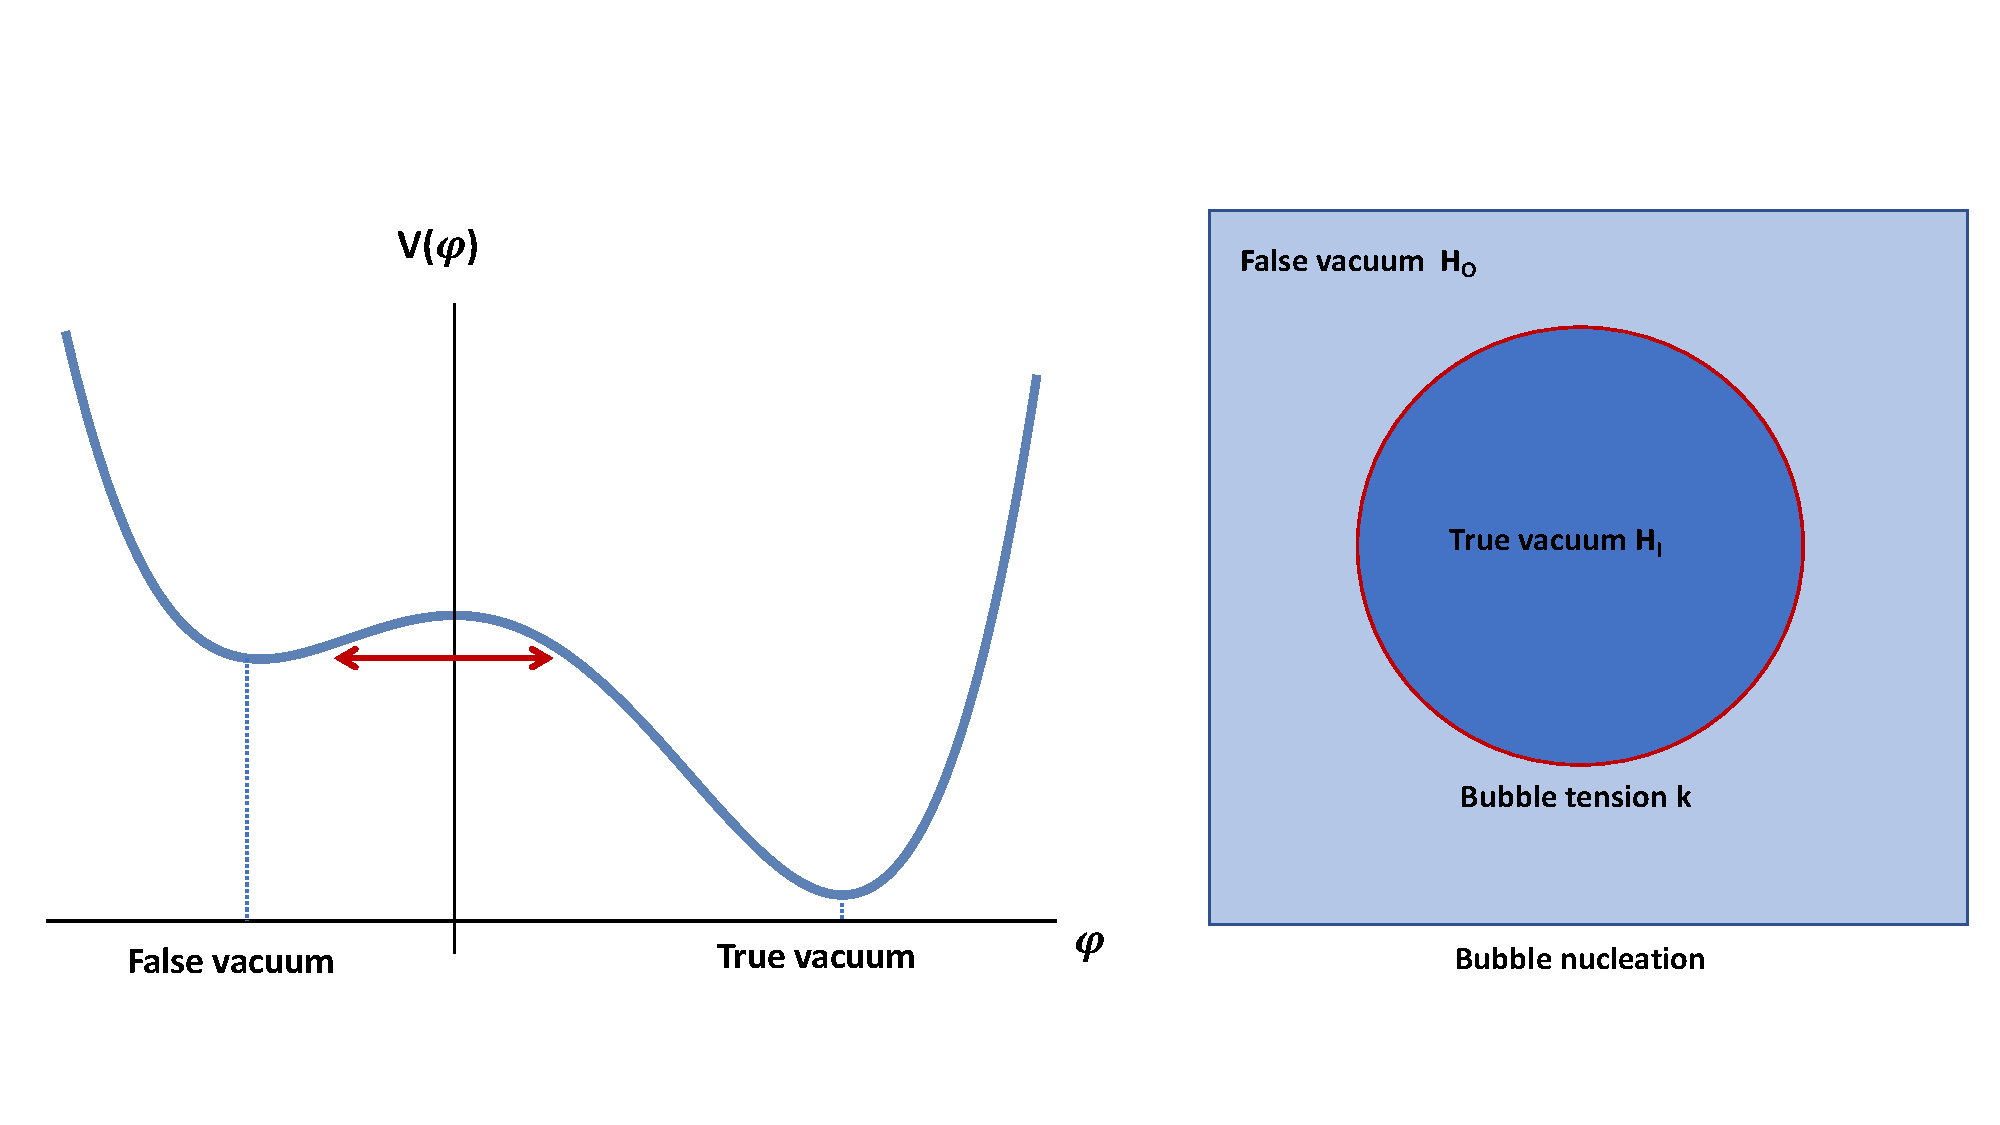
\includegraphics[width = 0.9\textwidth]{Sections/Figures/VacuumTransition.pdf} 
\caption{Bubble nucleation for a transition from a false to a true vacuum. The opposite transition is also allowed as long as the two spaces are dS.}
\label{fig:BubbleNucleation}
\end{figure}

\subsubsection{The anthropic principle and the string theory landscape}
\label{ssec:landscape}

Even without any microscopic understanding to hand, our very existence suggests that the cancellation of vacuum energy has to occur. If the vacuum energy were positive and much larger than the observed value, the growth of structure would have ceased too early preventing the formation of galaxies. If it were much larger and negative, the universe would have already collapsed in a Big Crunch. Remarkably, Weinberg \cite{Weinberg2} arrived at the \emph{prediction} that the vacuum energy must be small and of the same order as the matter energy density using this anthropic argument with bound:\footnote{Although note that cosmological constants much larger than the observed value were already known to be excluded.}
\begin{equation}
\setlength\fboxsep{0.25cm}
\setlength\fboxrule{0.4pt}
\boxed{
-10^{-123} M_{\rm Pl}^4 \lesssim \rho_\Lambda \lesssim 3 \times 10^{-121} M_{\rm Pl}^4 \,. 
}
\label{E:Weinwin}
\end{equation}
If one assumes that observers require galaxies, and that observers typically evolve soon after galaxy formation, then the \emph{Why Now?} problem is also solved, as allowing the vacuum energy to be as large as possible whilst allowing for galaxy formation places it in line with the matter energy density directly after galaxy formation.  For the argument to be complete, one also requires a theory to produce a multitude of vacua, including ones with anthropically viable total vacuum energies, and a mechanism to populate them all. This is what the string theory landscape \cite{Susskind:2003kw} is proposed to provide.

As reviewed in Sec. 3, string theory has a (probably finite \cite{Douglas:2003um, Ashok:2003gk} but) enormous number of solutions corresponding to 4-dimensional spacetimes at low energies, which we call the \emph{string theory landscape}. Each solution has a number of distinct contributions to the vacuum energy.  The value of the moduli potential energy discussed in Sec. 3 (which incorporates classical and leading order perturbative and/or non-perturbative effects) is one such contribution. To these should be added subleading quantum corrections in both the $g_s$ and $\alpha'$ expansions, amongst which those at $\mathcal{O}(\alpha'^0)$ incorporate standard field theory loops. By considering a string-inspired simplified model of such a setup, Bousso and Polchinski \cite{Bousso:2000xa} argued that the string theory landscape accommodates a discrete set of total vacuum energies that are sufficiently densely packed in Planck units to include the observed dark energy, and that moreover, all the corresponding vacua can be populated via an eternal inflation driven by non-perturbative bubble nucleation.

The discreteness of the distribution of vacuum energies arises from the topological nature of the input parameters for string compactifications -- flux quanta, D-brane and other localised source numbers, and an internal manifold characterised by its Hodge numbers -- which all contribute directly and indirectly to the vacuum energy.  Building on earlier work by Abbott \cite{Abbott:1984qf} and Brown and Teitelboim \cite{Brown:1987dd,Brown:1988kg}, Bousso and Polchinski \cite{Bousso:2000xa} (see also \cite{Bousso:2007gp} for a review) considered in particular the vacuum energy contribution from a set of $J$ 4-form background fluxes. In analogy to the electromagnetic field, each 4-form field-strength, $F_{(i)}$, is quantised in units of its source membrane's `electric'-charge $q_i$, $F_{(i)}^{mnpq} = n_i q_i \epsilon^{mnpq}$, and gives a positive vacuum energy contribution
\begin{equation}
\rho_{\rm 4-form} = \frac12 \sum_{i=1}^J n_i^2 q_i^2 \,.
\end{equation}
Crucially, the background 4-form fluxes are unstable to non-perturbative tunnelling effects described by Euclidean instantons, in analogy to how an electric field between two oppositely charged parallel capacitor plates discharges via Schwinger pair creation of electron and positrons, in the case of a 4-form, the depletion occurs via the spontaneous appearance of spherical membranes. Inside the membrane, the associated field strength is lowered by one unit of membrane charge: $n_iq_i \rightarrow (n_i-1)q_i$, with a subsequent reduction in energy, $(n_i-\frac12)q_i^2$ balanced by the initial mass of the membrane, which then expands outwards at the speed of light; see Fig. \ref{fig:BubbleNucleation}.  If one separates the total vacuum energy into the 4-form flux contributions and all the rest (which we may call the `bare' cosmological constant),
\begin{equation}
\rho_{\Lambda} = \lambda + \frac12 \sum_{i=1}^J n_i^2 q_i^2\,,
\end{equation}
it takes an exponentially long time for the
the background fluxes to deplete and so their vacuum energy contribution could eventually cancel an order one bare cosmological constant, $\lambda<0$, to give a total $\rho_\Lambda$ within the Weinberg window (\ref{E:Weinwin}).  This fine cancellation requires:
\begin{equation}
2|\lambda| \lesssim \sum_{i=1}^J n_i^2 q_i^2 \lesssim 2(|\lambda| + 10^{-118})\,.
\end{equation}
That this is possible for charges not much less than one relies on the fact that there are multiple distinct 4-form fluxes and associated membranes (see Fig. 1 from \cite{Bousso:2000xa}). These arise from M/string-theory compactifications as high-dimensional forms and branes, such as 5-branes wrapping distinct 3-cycles in the internal space. For example, an internal manifold with $\sim 500$ 3-cycles, with flux numbers ranging up to say $9$, would give $\sim 10^{500}$ different vacua for the construction. 

Whilst the Bousso-Polchinski toy model captures much of the physics of the landscape, realistic string constructions require further considerations \cite{Denef:2007pq}: moduli have to be stabilised; fluxes backreact on the geometry so that the bare cosmological constant $\lambda$ and charges $q_i$ themselves depend on the flux integers, leaving the cosmological constant to vary in unpredictable ways; the types and numbers of fluxes and branes that can be included are constrained by charge conservation or tadpole cancellation.  More sophisticated studies of the distributions of supersymmetric and non-supersymmetric Calabi-Yau flux compactifications of various string theories were carried out in \cite{Denef:2004ze, Douglas:2003um, Ashok:2003gk, Dienes:2006ut}. A recent development in this direction is the incorporation of K\"ahler moduli stabilisation, thereby ensuring that the sampling is only over the minima of the moduli potential (see e.g. \cite{Broeckel:2020fdz, Cicoli:2022chj} and references therein). Constructions with as many as $10^{272\,000}$ vacua have been proposed \cite{Taylor:2015xtz}, while F-theory models of dark energy have been proposed in \cite{Heckman:2019dsj, Heckman:2018mxl}.

In summary, string theory plausibly contains a landscape of vacua with a dense spectrum of vacuum energies that includes the observed vacuum energy, and a mechanism to populate them via membrane nucleation. The cosmological history of this scenario assumes that the universe starts with a large positive vacuum energy, expanding exponentially as dS space.  Eventually, somewhere within the universe, a membrane bubble will nucleate within which there is a lower vacuum energy.  This bubble will grow, but not as fast as the initial vacuum expands, the latter providing an ambient `multiverse'. Thus a process of eternal inflation ensues, with bubble nucleation continuing inside and outside existing bubbles, each bubble containing a long-lived open FRW universe and each jump in vacuum energy being not much smaller than one in Planck units, allowing for the creation of hot and dense universes. Eventually, one such bubble nucleation will create an anthropic universe, with the vacuum energy lowered to within the Weinberg range (\ref{E:Weinwin}) where the Big Bang begins.  See Fig. \ref{fig:Multiverse}.


\begin{figure}[ht]
    \centering
    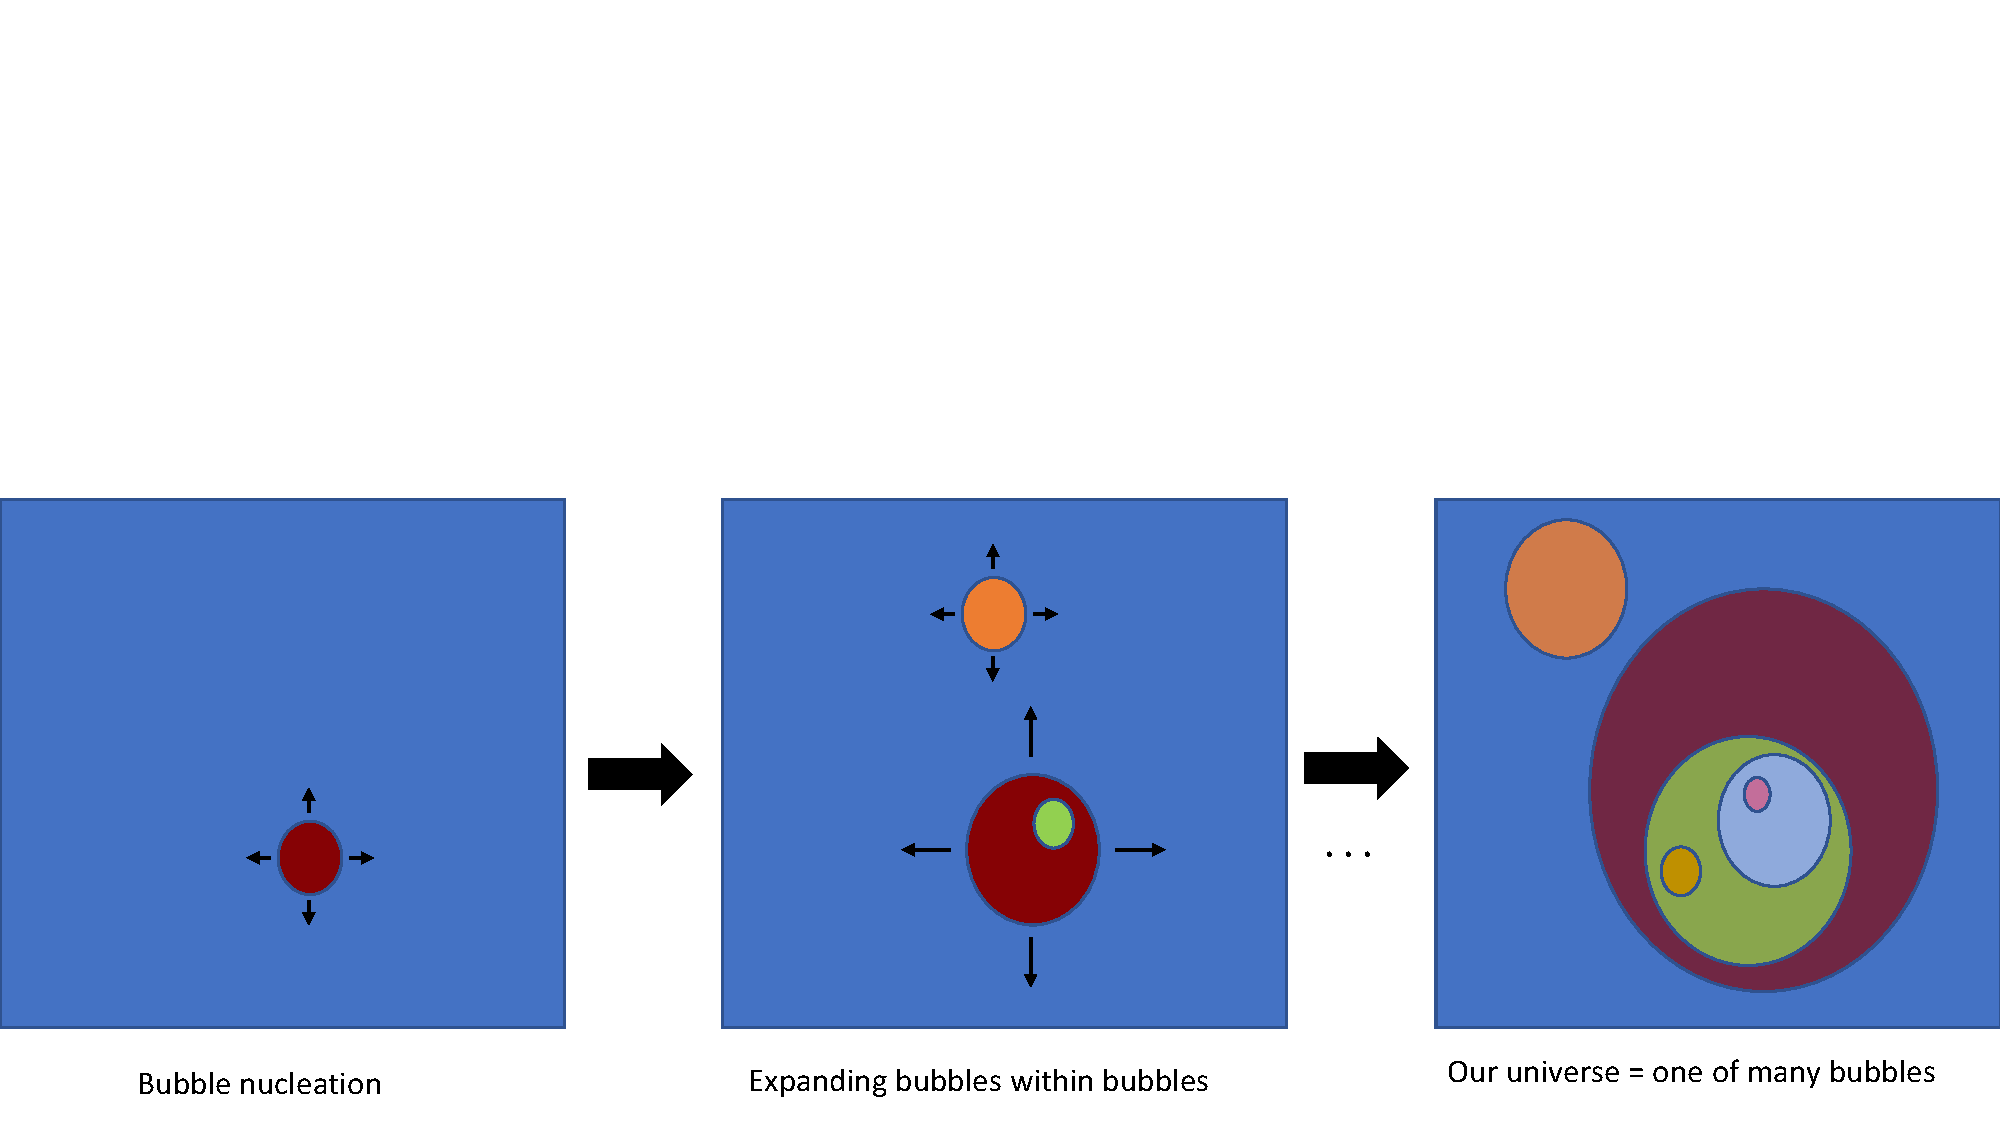
\includegraphics[width = 0.99\textwidth]{Sections/Figures/Figure_Multiverse_3.pdf} 
    \caption{Multiverse obtained by the process of bubble nucleation due to vacuum transitions from one dS vacuum to another with different cosmological constant.}
    \label{fig:Multiverse}
\end{figure}

\subsubsection{Open questions on the landscape}

The proposal of the string theory multiverse is deeply controversial. If true, it would motivates a paradigm shift in answer to the cosmological constant problem -- the value of the cosmological constant is environmental and our very existence implies it must happen to fall within the Weinberg range in our patch of the multiverse. In this case, there seems no reason to expect any further microscopic explanation at play. However, there remains work to be done.

Essential to the string theory landscape is an understanding of moduli stabilisation, reviewed in Sec. \ref{sec:MS}. So far, there are few attempts at achieving simultaneously moduli stabilisation and the Standard Model of particle physics (see \cite{Cicoli:2021dhg} for some recent progress). A complete model must (of course) include the vacuum energy of the Standard Model and dark matter amongst all the different contributions to be anthropically cancelled. 

To be more concrete, however, consider the simplified type IIB moduli stabilisation scenarios of KKLT and LVS. It is important to recognise that, although we can aim to make well-controlled dS vacua and -- remarkably -- even compute to good precision the vacuum energy in the weak coupling, weak curvature expansions, we cannot hope -- with current technology -- to obtain an explicit construction with fine-tuned vacuum energy $\mathcal{O}(10^{-120})$. The interplay between various classical and quantum effects are argued to give rise to metastable dS vacua, with the effective parameters such as $W_0$, $A$ and $a$ in $W =W_0+ A \, e^{-aT}$ (see Sec.~\ref{sec:MS}), ultimately depending on topological numbers such as flux integers and numbers of branes or instantons. The first obstacle arises from the difficulty to determine the exact dependence of parameters like $W_0$ and $A$ on the complex structure moduli and the explicit stabilisation of these moduli in terms of the discrete microscopic parameters. Moreover, even if discretely adjusting these integers allowed the effective parameters to be finely-tuned to give an anthropically viable metastable vacuum at weak coupling and large volume, the fine-tuning would typically be spoilt by higher order $g_s$ and $\alpha'$ corrections to the vacuum energy. To illustrate this point with a very simple toy model, consider a one-modulus system with canonical kinetic term and a scalar potential using an expansion in small $\phi$:
\begin{equation}
V(\phi) = \left(a_0 + a_2 \phi^2 + a_3 \phi^3 + a_4 \phi^4 + \dots\right)  \,.
\end{equation}
Assuming some mild hierarchy in the parameters $|a_3| \gg |a_i|$, $i\neq 3$, and $a_2 <0$, induces a metastable minimum $\langle \phi \rangle = -\frac{2 a_2}{a_3} \ll 1$ consistent with the expansion. If we assume that the leading coefficients are fine-tuned such that 
$$a_0-\frac{4}{27}\left(\frac{|a_2|^3}{a_3^2} \right) \sim 10^{-120},$$ 
then without further fine-tuning the higher order contributions $\mathcal{O}\left( \phi^4 \right)$ to the vacuum energy will dominate. Thus it is the full vacuum energy, including Standard Model/dark matter contributions and all $g_s$ and $\alpha'$ corrections -- right up to the order where the corrections are suppressed down to $10^{-120}\,M_{\rm Pl}^4$ without fine-tuning --  that has to be anthropically fine-tuned. This arguably weakens the significance of the challenges in uplifting the leading order AdS vacua of moduli stabilisation scenarios to dS (see \cite{deAlwis:2021zab}), although notice that the Standard Model contributions to the vacuum energy were found to be negative in \cite{Koksma:2011cq,Martin:2012bt}. Nevertheless, the key that the string landscape offers is the realisation that flux vacua lead to a finely-spaced distribution of vacuum energies over a suitably large range; even if the other contributions move this distribution up or down in energy, one may still expect vacuum energies of order of the observed dark energy amongst the final vacua.

Weinberg's anthropic window was derived by assuming that all other Standard Model parameters are fixed to their observed values. However, the string landscape suggests that all of these parameters would similarly vary from vacuum to vacuum.  For example, if effective field theory parameters are such that primordial density perturbations are larger or grow faster, anthropic arguments would require a larger positive vacuum energy. It is not yet clear how to use this framework to make predictions. Any statistical approach (see \cite{Denef:2004ze, Douglas:2003um, Broeckel:2020fdz, Broeckel:2021dpz, Cicoli:2022chj} and \cite{Kumar:2006tn} for a pedagogical review), by searching for those properties which have probability $\sim\mathcal{O}(1)$ in the landscape (see \cite{Page:2007bt, Hartle:2007zv} for discussions for and against our typicality) or identifying distinct low-energy features that are strongly correlated, would require an understanding of the measure on the space of vacua. Such a measure would need to include consideration of the dynamical mechanism that populates the landscape, which may prefer some vacua over others. This connects to the measure problem of eternal inflation, where bubbles of open universes with infinite spatial extent, reproduced infinitely many times, pose ambiguities in how to regularise \cite{Linde:1993xx, Guth:2000ka}.  

For some recent progress on searching the string landscape for models with phenomenological features using machine learning techniques see \cite{Cole:2021nnt}. Another strategy is to understand which classes of effective field theory can be consistently embedded into the string theory landscape (i.e. have a consistent UV completion into quantum gravity), and which classes instead lie in the swampland with no UV completion incorporating gravity \cite{Vafa:2005ui}. In fact, there are several conceptual challenges posed by any quantum theory on dS spacetime \cite{Witten:2001kn, Banks:2012hx, Maltz:2016iaw, Dvali:2018jhn}, most notably the absence of a well-defined S-matrix. Together with the technical challenges in achieving explicit, well-controlled moduli stabilisation with metastable dS vacua, this has led to the provocative conjecture that long-lived metastable dS vacua may actually lie in the swampland \cite{Garg:2018reu,Ooguri:2018wrx}. Although `may' does a lot of work in this last sentence, even if such a conjecture were true, it may still be of course reasonable to expect that our observed universe is sufficiently short-lived to stay in the landscape.

The landscape's approach to dark energy has led to several general proposals for combining it with the physics of vacuum transitions, a period of inflation, bubble collisions, etc. In particular, the general claim  that CDL vacuum transitions give rise to open universes after bubble nucleation has given rise to a holographic scenario for eternal inflation. See for instance \cite{Freivogel:2006xu,Sekino:2009kv}. For recent discussions to address the vacuum selection in terms of self-organised criticality see \cite{Kartvelishvili:2020thd,Giudice:2021viw}.

\subsection{Dynamical Dark Energy/Quintessence in String Theory}

In the previous section we discussed dS vacua in the string theory landscape as a possible explanation to present day accelerated expansion of the universe. However, given the debates around this proposal and observational prospects of measuring the dark energy equation of state and its time dependence, it is important to consider alternatives. The main alternative to a vacuum energy is a scalar field that is slow-rolling at positive energies, thus driving the accelerated expansion. This scenario goes under the generic name of {\em quintessence} \cite{Ratra:1987rm,Caldwell:1997ii} and much of the physics is similar to that of cosmic inflation, discussed in Sec. 4.
During quintessence, the equation of state of dark energy changes with time, similarly to inflationary cosmology, though initially Hubble friction can keep the field frozen yielding an effective cosmological constant. Quintessence scenarios with exponential or inverse power-law potentials are particularly attractive because they lead to equations of motion with attractor behaviour \cite{Ratra:1987rm} such that the present-day accelerated expansion is independent of the initial conditions. Moreover, these attractor solutions are usually scaling solutions such that the energy density scales as a power of the scale factor, and -- for the inverse power-law potentials -- the scalar field energy density can scale more slowly than the background fluid, allowing it to dominate eventually and drive the accelerated expansion \cite{Liddle:1998xm}.
 
Scalar fields abound in string theory and so it might seem rather natural to expect that one of them is at present rolling towards its minimum at a finite or infinite value. Among the scalar fields present in string theory, we can identify several potential candidates for quintessence: closed and open string string moduli, axions and runaway moduli. Moreover, scenarios where more than one scalar field drive the present day acceleration are also possible, as well as models of coupled dark sectors, where the dark energy and dark matter sectors are coupled. Time-dependent compactifications of the 10/11-dimensional supergravities that descend from string theory are also known to include accelerating cosmologies.

After reviewing the major challenges in the quintessence scenario, we will discuss each candidate in turn. 


\subsubsection{Challenges for quintessence}
\label{sec:ChallengesQ}

Any quintessence scenario must meet a number of theoretical and observational challenges. Some of these are common to all quintessence models, irrespective of any string theory embedding (see \cite{Kolda:1998wq} for a review of phenomenological scenarios):
\begin{itemize}
\item \emph{Cosmological Constant Problem} -- quintessence scenarios start by assuming that some unknown mechanism fixes the background vacuum energy to zero, on top of which the quintessence dynamics plays out to drive the accelerated expansion. The symmetries that are known to do this job, e.g. supersymmetry or conformal symmetry, only work down to scales much higher than the observed vacuum energy, around the TeV scale, where they must be broken, although one exception may be the approximate shift symmetry associated with a pseudo-Goldstone boson \cite{Weinberg:1972fn}. The cosmological constant problem is the big elephant in the room of any quintessence construction. 

\item \emph{Radiative corrections to quintessence mass} -- for quintessence to drive an accelerated expansion, the quintessence scalar mass must be sufficiently light; $m_q \lesssim H_0$ with today's Hubble constant $H_0 \sim 10^{-33}$ eV.  On the other hand, as a scalar field, the quintessence mass is sensitive to quantum loops and -- in a similar way to the Higgs boson -- would be driven up to the UV cutoff. Again, symmetries like supersymmetry and conformal symmetry could help only down to TeV scales.  

\item \emph{`Why Now?' problem} -- Given the different scaling properties of radiation, matter and dark energy densities with the cosmological scale factor, $a(t)$, the current epoch -- in which all three of the energy densities are of the same order -- seems very special. Why does there exist an epoch in which all three densities are comparable, and why do we happen to live in this epoch? In quintessence models, the scalar field equation of motion may admit `tracker' solutions, in which the pressure and energy density in the scalar field tracks that of the dominant energy density \cite{Zlatev:1998tr, Steinhardt:1999nw}. Moreover, these tracker solutions may be late-time attractors, and hence be reached independently of the initial conditions.  However, in order for dark energy to come to dominate, the evolution must depart from the tracker solution so that the field ends up locked at an approximately constant value. To achieve this at the right time would seem to require some overall fine-tuning.

\item \emph{Fifth forces} -- Being a light boson, the quintessence field mediates long-range fifth forces. Current constraints \cite{Adelberger:2003zx} indicate that any scalar with mass less than around the meV scale must have weaker than Planckian couplings to the Standard Model. This would appear to rule out using one of the universal string moduli, such as the volume modulus or dilaton, as the quintessence field since these moduli couple to all fields with Planckian strength after Weyl rescaling to the Einstein frame. Note that even if such fields were to couple universally to matter, they would not simply lead to a renormalisation of Newton's constant as the nature of a spin-0 force is distinct from the nature of a spin-2 force. Non-universal moduli typically have couplings to the Standard Model that violate the equivalence principle, and such couplings are phenomenologically constrained to be at least a factor $10^{-11}$ weaker than gravity \cite{Damour:2010rp}. 
    
Another proposal is that fifth forces are screened in high ambient matter densities such as close to the Earth, due to non-minimal couplings to matter and/or certain derivative or non-derivative self-interactions \cite{Vainshtein:1972sx, Khoury:2003aq, Feldman:2006wg, Hinterbichler:2010es} (see \cite{Brax:2010gi, Hinterbichler:2010wu} for work towards embedding these mechanisms into string theory).  
    
Finally, pseudoscalars such as string axions, coupling as they do via derivative axial-current interactions of the form $\partial_\mu \theta (\bar{\psi} \gamma^\mu \gamma_5 \psi)$, need spin-polarised sources in order to be detectable via fifth forces and so evade fifth-force experiments using macroscopic bodies (searches for new mass-spin couplings are reviewed in \cite{Marsh:2015xka, Workman:2022ynf} with the strongest constraints coming from stellar cooling \cite{Raffelt:2012sp}, still far from the parameter space of quintessence).  In fact, axions can also be used to help screen scalar fifth forces \cite{Burgess:2021qti,Brax:2022vlf}; the non-linear target-space interactions between axions and saxions that typically appear in string constructions might convert would-be dilaton profiles to axion profiles, which can then be probed only by axion-matter couplings rather than dilaton-matter couplings. 

\item \emph{Time variation of fundamental constants} --  if quintessence is a string modulus that sets the visible sector gauge kinetic functions, Yukawa couplings or Planck mass, then its rolling would lead to unobserved time-variation of the fundamental constants. Similarly to fifth forces, this disfavours closed string moduli like the volume or dilaton as quintessence.  The problem may be reduced by using a local modulus geometrically sequestered from the visible sector. 

\end{itemize}
Quintessence models must also satisfy observational constraints, not just on the equation of state $w$ but also on compatibility with local $H_0$ measurements (for example, see
\cite{Colgain:2019joh, Banerjee:2020xcn, Lee:2022cyh, Heisenberg:2022lob, Heisenberg:2022gqk,Colgain:2022rxy} for recent discussions).

In addition to these overarching questions common to all quintessence scenarios, there are also a number of issues specific to string theoretic models:
\begin{itemize}
\item \emph{Moduli stabilisation problem} -- even supposing a light ($m_q \lesssim H_0 \sim 10^{-60}\,M_{\rm Pl}$), slowly-rolling modulus can be identified, all other moduli must be safely stabilised in a way compatible with the string mass above the TeV-scale (see \cite{Hebecker:2019csg} for a recent discussion). Given constraints from fifth-forces and time variation of fundamental constants, the stabilised moduli must include the overall volume modulus and the dilaton with $m \gtrsim 10^{-30}\,M_{\rm Pl}$, which increases to $m \gtrsim 10^{-14}\,M_{\rm Pl}$ when the cosmological moduli problem is taken into account. Possible quintessence candidates are then ratios of K\"ahler moduli or blow-up moduli that (hardly) affect the overall volume, complex structure moduli or axions. Moreover $M_{\rm soft} \gtrsim 10^{-15}\,M_{\rm Pl}$ from the absence of sparticles at the LHC, and $M_{\rm KK} \gtrsim 10^{-30}\,M_{\rm Pl}$ from tests of Newton's inverse square law (see \cite{Hebecker:2019csg} for further discussion in the context of the Large Volume Scenario, where the volume modulus may be used to suppress scales but is then also too light itself).

These phenomenological requirements imply a large hierarchy between the potential which stabilises the volume modulus $\mathcal{V}$, $V_0(\mathcal{V})$, and the one for the quintessence field $\phi$, $V_1(\mathcal{V},\phi)$ (recall the volume modulus couples to everything) \cite{Cicoli:2021skd}. In fact, the total dark energy potential should look like
\begin{equation}
V_{\rm DE}\simeq V_0(\mathcal{V}_{\rm min})+V_1(\mathcal{V}_{\rm min}, \phi)\simeq V_1(\mathcal{V}_{\rm min}, \phi)\,,
\end{equation}
where $\mathcal{V}$ needs to stabilised in a near-Minkowski vacuum, $V_0(\mathcal{V}_{\rm min}) \sim 0$, since $V_1$ is a tiny correction with respect to $V_0$ to guarantee that the mass of the volume mode is at least above the meV-scale while $m_q \sim 10^{-32}$ eV, and so a leading order stabilisation in an AdS vacuum would remain AdS even after adding $V_1$. Thus we require
\begin{equation}
\frac{V_1(\mathcal{V}_{\rm min}, \phi)}{V_0(\mathcal{V}_{\rm max})} \sim \left(\frac{m_q}{m_{\mathcal{V}}}\right)^2\lesssim 10^{-60}\,,
\label{QuintHierarchy}
\end{equation}
where $V_0(\mathcal{V}_{\rm max})$ is the value of $V_0$ at the potential barrier towards decompactification. Note that this is a huge hierarchy, which can hardly be obtained if both $V_0$ and $V_1$ are generated by perturbative corrections since it would require values of $\mathcal{V}$ too large to ensure $M_s\gtrsim 1$ TeV. As an illustrative example consider LVS models where $\mathcal{V}$ is fixed by $\mathcal{O}(\alpha'^3)$ effects which therefore set the size of $V_0$. If $\phi$ is a fibre modulus different from the inflaton, its potential would be generated by $\mathcal{O}(g_s^2 \alpha'^4)$ string loops which would set the size of $V_1$, yielding:
\begin{equation}
\frac{V_1}{V_0} \sim \frac{V_{g_s^2 \alpha'^4}}{V_{\alpha'^3}} \sim \frac{1}{\mathcal{V}^{1/3}}\lesssim 10^{-60}\qquad \Leftrightarrow\qquad 
\mathcal{V}\gtrsim 10^{180}\,,
\end{equation}
which would imply an extremely low string scale $M_s \sim M_{\rm Pl}/\sqrt{\mathcal{V}}\ll 1$ TeV. This shows that constructing a scalar potential with the hierarchy of scales as in (\ref{QuintHierarchy}) is a challenge. Note that in models where $\mathcal{V}$ does not evolve from inflation to today, this hierarchy could be even larger since preventing volume destabilisation during inflation (a quintessence version of the Kallosh-Linde problem) requires $\left(V_1/V_0\right)\lesssim \left(H_0/H_{\rm inf}\right)^2$. Depending on the inflationary scale, this yields $10^{-108}\lesssim \left(V_1/V_0\right)\lesssim 10^{-36}$ \cite{Cicoli:2021skd}. As pointed out in \cite{Cicoli:2021skd}, a natural way to achieve this huge hierarchy could be to fix $\mathcal{V}$ by perturbative effects, and then use axions as quintessence fields since their potential is generated by exponentially suppressed non-perturbative effects. Being axions, they also naturally avoid fifth-force problems, and their shift symmetry guarantees the radiative stability of the quintessence field mass. 
   
\item \emph{F-term problem} -- This is a rephrasing of the cosmological constant problem for quintessence models in the context of LVS moduli stabilisation \cite{Hebecker:2019csg}. The supersymmetry breaking in the Standard Model sector, say localised on some brane configuration, gives a large positive contribution to the scalar potential, $\delta V_{sb} \sim M^2 M_{\rm soft}^2 \sim 10^{-60}\,M_{\rm Pl}^4$, where $M$ is the mediation scale with $M\gtrsim 10^{-15}\,M_{\rm Pl}$. Clearly, in the absence of a source to cancel this large contribution, the vacuum energy would be way beyond the dark energy scale (see \cite{Cicoli:2012tz} for a scenario in which this large vacuum energy is supposed to finely cancel against contributions from the backreaction of non-supersymmetric visible sector branes). More generally, after supersymmetry breaking, the mass of the quintessence field would typically be of order the gravitino mass (see \cite{Chiang:2018jdg} and \cite{Cicoli:2018kdo} for some ways to evade this).
    
\item \emph{Sequestering in supergravity} -- Within the context of 4-dimensional $N=1$ supergravity, the usual low-energy description of string compactifications, it is difficult to suppress couplings between the quintessence field and Standard Model degrees of freedom such as the Higgs \cite{Denef:2018etk, Cicoli:2018kdo}. The scalar potential has to take the form 
\begin{equation}
V(\Phi, \chi)=e^{K(\Phi, \chi)}(|D_\chi W|^2 + |D_\Phi W|^2 - 3|W|^2),
\end{equation}
with $\Phi$ the quintessence superfield and $\chi$ denoting (collectively) the matter superfields. Assuming a maximal decoupling with K\"ahler potential and superpotential taking the form 
\begin{equation}
K=K_q(\Phi)+K_m(\chi),
\end{equation}
and 
\begin{equation}
W=W_q(\Phi) + W_m(\chi),
\end{equation}
and moreover taking a canonical normalisation $K_q = \Phi \bar{\Phi}$ and e.g. $W_q=\frac{2}{\beta}\sqrt{\Lambda} e^{-\frac12 \beta \Phi}$ so that \begin{equation}
V\sim \Lambda e^{-\beta \phi},
\end{equation}
one obtains couplings of the form 
\begin{equation}
\delta V \sim \frac{\bar{\Phi}_0}{M_{\rm Pl}^2} \delta\Phi |D_\chi W|^2, \qquad \delta \mathcal{L} \sim \frac{\bar{\Phi}_0}{M_{\rm Pl}^2} \delta\Phi \mathcal{L}_{\rm fermion}, \qquad \delta \mathcal{L} \sim -\frac{3T(G)}{16\pi^2} \frac{\Phi_0}{M_{\rm Pl}^2} \delta \Phi \mathcal{L}_{\rm gauge},
\end{equation}
(where $T(G)$ is a group theory number). 

Even if we choose $\Phi_0=0$ to evade present fifth forces constraints, at some point in the past we would have had $\Phi_0 \sim \mathcal{O}(1)M_{\rm Pl}$, giving Planck suppressed linear couplings between the quintessence field and the Standard Model for which there are strong bounds (see \cite{Chiang:2018jdg} for a recent example of quintessence model in supergravity). 

The most obvious way to try to achieve sequestering is to consider quintessence as an open string modulus geometrically separated from an open string realisation of the Standard Model, for which the K\"ahler potential takes the form 
\begin{equation}
K = -3M_{\rm Pl}^2 \ln \left( 1 - \frac{f(\Phi, \bar\Phi)}{3 M_{\rm Pl}^2} - \frac{g(\chi, \bar\chi)}{3M_{\rm Pl}^2} \right).
\end{equation}
It is not yet clear if sufficient coupling suppression can be achieved (see \cite{Conlon:2007gk, Cicoli:2010ha, Cicoli:2012cy, Abel:2008ai, Burgess:2008ri, Goodsell:2009xc, Cicoli:2011yh, Gan:2023wnp} for some stringy mechanisms of kinetic mixing, \cite{Berg:2010ha} for a summary of the challenges, \cite{Aparicio:2014wxa} for some proposed solutions and \cite{Acharya:2018deu} for some recent progress including a lower bound on the volume modulus to suppress the couplings between the Standard Model and other K\"ahler moduli).  
\end{itemize}
     



\subsubsection{Runaway quintessence -- single field} 
\label{S:singlefieldq}

The vast moduli sector of string compactifications offers the ideal place to look for quintessence candidates. Given the ubiquity of runaway moduli in string compactifications (see discussion on the Dine-Seiberg problem in Sec. 3), one may expect runaway quintessence scenarios to be easily realised, without the need for delicate interplay between various not-so-under-control ingredients as in dS vacua. As string moduli usually correspond to low energy couplings or expansion parameters, by setting up moduli to be slowly-rolling close to their asymptotic regime, parametric control\footnote{The expansion can be made arbitrarily good by making the expansion parameter arbitrarily small.} of expansions could be ensured with, moreover, a naturally suppressed vacuum energy.  Phenomenological bounds on the parameter $\lambda$ for runaway scalar potentials of the form $V(\phi) \sim V_0\,e^{-\lambda\phi}$ were found to be $\lambda \lesssim 1.02$ and $\lambda \lesssim 0.6$ at 3$\sigma$ in \cite{Akrami:2018ylq} and \cite{Agrawal:2018own}, respectively.

As mentioned above, the first candidate runaway moduli that one may think of are the overall volume and the dilaton since they are model independent; rolling towards infinite volume or zero coupling, respectively, in the asymptotic limit. Indeed, the dilaton was used early on as a quintessence candidate in \cite{Gasperini:2001pc,Damour:2002mi}, although ref. \cite{Cicoli:2021fsd} has recently shown that runaways for the volume mode and the dilaton at tree-level, where one could in principle achieve parametric control over all approximations, are never flat enough to drive an epoch of accelerated expansion. Nevertheless, the main difficulty with these moduli is that they couple to all matter fields. The strong bounds on fifth-forces and varying constants thus make these options untenable. On the other hand, if the runaway direction is a local modulus in a hidden sector it may plausibly avoid constraints from fifth forces and time variation of fundamental constants. Yet as we now discuss, even before worrying about these phenomenological challenges, it turns out to be intriguingly difficult to identify runaway directions in string theory that are sufficiently flat to source the required acceleration \cite{Olguin-Tejo:2018pfq,Bento:2020fxj}.  

For example, consider for simplicity a moduli stabilisation scenario in which all but one of the moduli are stabilised as heavy fields in a supersymmetric Minkowski vacuum. The remaining supersymmetric flat direction $\Phi$ is protected by non-renormalisation theorems \cite{Dine:1986vd}, but is ultimately lifted by non-perturbative effects. If this is a bulk modulus, it will typically have a K\"ahler potential and superpotential of the form:
\begin{equation}
\setlength\fboxsep{0.25cm}
\setlength\fboxrule{0.4pt}
\boxed{
K = -p\ln(\Phi + \bar{\Phi}) \qquad\textrm{and}\qquad W = A\, e^{-a\Phi} 
\label{E:DSrunaway}
}
\end{equation}
for some constants $p, A, a$. The resulting scalar potential for the saxion $\phi = {\rm Re}(\Phi)$, with runaway towards $\phi \rightarrow \infty$ is plotted in Fig. \ref{F:runaways} for $p=1,3$, and it is easily shown that the slow-roll parameter diverges at the tail:
\begin{equation}
\setlength\fboxsep{0.25cm}
\setlength\fboxrule{0.4pt}
\boxed{
\epsilon_V \rightarrow \frac{4}{p} a^2 \phi^2 \qquad\text{as}\qquad \phi \rightarrow \infty,
}
\end{equation}
and thus this potential is always too steep to drive an accelerated expansion \cite{Olguin-Tejo:2018pfq}.  

\begin{figure}[ht]
\centering
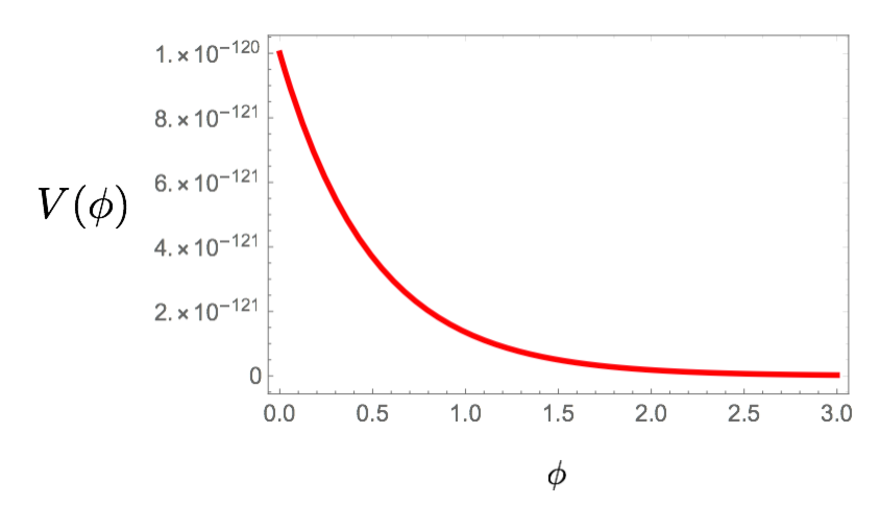
\includegraphics[width = 0.45\textwidth]{Sections/Figures/Runaway1.pdf} \qquad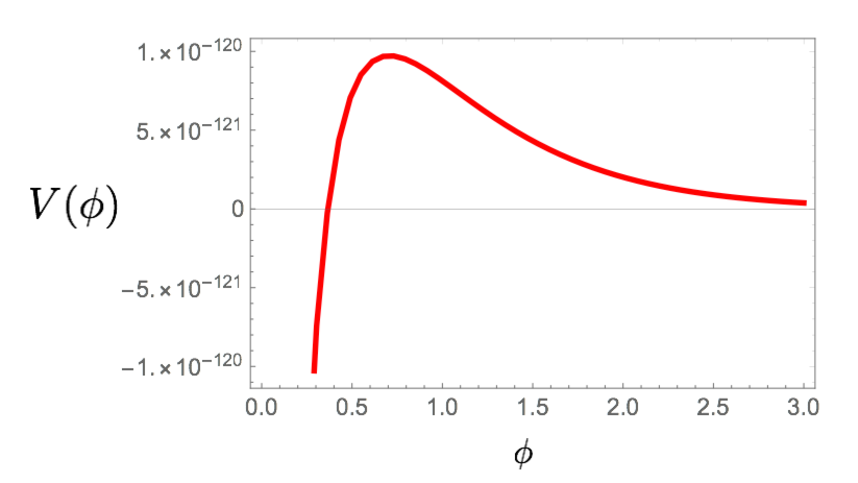
\includegraphics[width = 0.4\textwidth]{Sections/Figures/Runaway2.pdf}
\caption{Typical runaway potentials: the scalar potentials derived from eq. (\ref{E:DSrunaway}) for $p=3$ (left-hand side) and $p=1$ (right-hand side).}
\label{F:runaways}
\end{figure}

In fact, it has been shown using $N=1$ supergravity that all the typical string moduli -- whether bulk or local, whether lifted by perturbative or non-perturbative superpotentials -- have potentials that satisfy either $\epsilon_V > 1$ or $\rho_V < 0$ and so cannot drive an accelerated expansion, see Tab. \ref{quintrunnogos} \cite{Bento:2020fxj}. These results have been extended in \cite{Cicoli:2021fsd} considering no-scale models in type IIB, IIA and heterotic string compactifications. The limitations from string-inspired 4-dimensional $N=1$ supergravity on obtaining slow-roll potentials are reminiscent of similar results from \cite{Hellerman:2001yi} which show that, for a class of supersymmetric theories, it is impossible to relax into an asymptotic zero-energy supersymmetric minimum whilst accelerating (see also \cite{Rudelius:2021azq}). The theories considered are those with a single field with exponential potential $V\sim e^{-c\phi/M_{\rm Pl}}$; indeed, if the potential is to have a zero-energy supersymmetric vacuum and support $w_{\rm DE}={\rm constant}$ quintessence-like evolution, then it must have this form asymptotically, with $|c|< \sqrt{2}$. Assuming that the dynamics is indeed towards a zero-energy supersymmetric minimum at $\phi \rightarrow \infty$, Ref. \cite{Hellerman:2001yi} shows how 4-dimensional $N=1$ supersymmetry implies that having $V>0$ requires $c > \sqrt{6}$ and thus excludes slow-roll.   


\begin{table}[ht]
\begin{center}
\centering
\begin{tabular}{| c | c | c | c | c |}
\hline
{\cellcolor[gray]{0.9}$K$} & {\cellcolor[gray]{0.9}$W$} & {\cellcolor[gray]{0.9}$V>0 \quad \epsilon_V<1$} \\
\hline
\hline
$-p\ln(\Phi+\bar{\Phi})$ & $W_0 + A\,e^{-a\Phi}$ & no-go \\
\hline
$-p\ln(\Phi+\bar{\Phi})$ & $W_0 + A\,\Phi^n$ & no-go \\
\hline
$k_0 + \frac{|\Phi|^{2p}}{k_1}$ & $W_0 + A\,e^{-a\Phi}$  & no-go \\
\hline
$k_0 + \frac{|\Phi|^{2p}}{k_1}$ & $W_0 + A\,\Phi^n$ & no-go except for $p=n$ \\
\hline
$k_0 + \frac{(\Phi+\bar{\Phi})^{2p}}{k_1}$ & $W_0 + A\,e^{-a\Phi}$  & no-go \\
\hline
$k_0 + \frac{(\Phi+\bar{\Phi})^{2p}}{k_1}$ & $W_0 + A\,\Phi^n$ & no-go except for $p=n$ \\
\hline
\end{tabular}
\end{center} 
\caption{Summary of no-go theorems for string inspired supergravity models of single-field runaway quintessence, and parameter points that evade them. The K\"ahler potentials correspond, respectively, to bulk moduli, fibre moduli and blow-up moduli, and the superpotentials correspond to the flat direction $\Phi$ being lifted, respectively, by a leading non-perturbative effect or a leading perturbative one.  No-scale scenarios, having $K=-3\ln(\Phi + \bar{\Phi})$ and $W$ independent of $\Phi$, are included in the case that no-scale-breaking occurs via non-perturbative corrections to $W$.}  
\label{quintrunnogos}
\end{table}  

Note that we have -- as is usual in quintessence and as is entirely unsatisfactory in string theory -- left aside the cosmological constant problem and the fact that supersymmetry in the Standard Model sector must be broken at least at TeV scales which is clearly a challenge for supersymmetric vacua where the supersymmetry breaking scale would naturally be set by the dark energy scale.  At the same time, the difficulties in obtaining runaway directions that sustain accelerated expansion seem to extend to non-supersymmetric setups. The runaway potentials 
associated with NS-NS tadpoles in non-supersymmetric string theories are also too steep for quintessence, taking the form $V=\Lambda\, e^{-\gamma \phi}$ with $\gamma=\frac52, \frac32, \frac32$ in the Einstein frame, for the SO(16)$\times$SO(16) theory, the orientifold $USp(32)$ Sugimoto model, and the type 0B' model, respectively (see \cite{Basile:2020mpt} for an extension of dS no-go theorems to non-supersymmetric string theories).

These no-go theorems against single-field runaway quintessence support the conjecture against dS vacua, which are indeed best motivated at the asymptotic boundary of moduli space \cite{Ooguri:2018wrx}. However, as we will discuss in Sec. \ref{S:multiq}, there may be paths to 
evade these no-go results by considering multifield scenarios.

\subsubsection{Hilltop quintessence}

Alongside runaway moduli, which are ubiquitous in string compactifications, dS maxima are also very easy to find. For example, the Dine-Seiberg runaway potential in eq. (\ref{E:DSrunaway}) for $p=1$ is shown in Fig. \ref{F:runaways} to have a dS hilltop. In \cite{Olguin-Tejo:2018pfq}, the possibility of sourcing quintessence at the hilltop was explored (see \cite{Dutta:2008qn} for a phenomenological analysis of hilltop quintessence). If the modulus starts close to the hilltop, it can remain frozen there by Hubble friction for much of the cosmological history, first sourcing an effective cosmological constant and then turning into a rolling quintessence field with observable consequences. The parameters could be chosen to match the observed dark energy, consistent with the refined dS swampland conjecture (see Secs.~\ref{S:DEswamp} and \ref{Sec:Swamp} below) and with sub-Planckian field displacements. Quantum fluctuations $\Delta \varphi \sim H/(2\pi)$ leave the field within the viable window close to the hilltop until $H \sim 0.01\,M_{\rm Pl}$. Although there is no need for fine-tuning in the Lagrangian parameters, the fine-tuning of initial conditions is difficult to motivate, perhaps resorting to some anthropic danger in starting from a point in field space that leads into a steep runaway.

Of course this is just a scenario, and even if motivation for the initial conditions could be found, work would need to be done to embed it in a fully fledged string construction with moduli stabilisation and control over subleading corrections; in particular it may be a challenge to achieve sufficient sequestering to hide fifth forces, higher order instanton corrections may not be suppressed, and -- as is usual in quintessence scenarios -- the cosmological constant problem and vacuum contributions from the susy-breaking visible sector have not been addressed. Further attention to the hilltop scenario was given in \cite{Cicoli:2021skd}, using the dS maximum for the volume modulus in the KKLT scenario, where it was found that matching with the observed dark energy would require an unacceptably light gravitino and light volume modulus.


\subsubsection{Axions as quintessence}

Axions are arguably the most attractive quintessence candidates \cite{Kaloper:2008qs, Panda:2010uq, Choi:1999xn,Cicoli:2021skd} as ($i$) being pseudo-scalars they evade the most stringent spin-independent fifth force bounds; ($ii$) they enjoy approximate shift symmetries which restrict the allowed couplings and protect the axion mass and potential energy density, which are otherwise UV sensitive quantities; ($iii$) their potential is generated by exponentially suppressed non-perturbative effects which can naturally reproduce the required hierarchy between the dark energy potential and the potential which fixes the volume modulus at leading order (for example via perturbative effects which break supersymmetry spontaneously) guaranteeing $M_{\rm soft}\gtrsim 1$ TeV and $m_{\mathcal{V}}\gtrsim 1$ meV in a way compatible with $m_q \sim 10^{-32}$ eV. 

From the string theory point of view, a rather generic prediction is the existence of a 
large number of axions \cite{Green:1987mn, Banks:1996ea, Banks:2002sd, Svrcek:2006yi, Conlon:2006tq}  -- sometimes called an \emph{axiverse} \cite{Arvanitaki:2009fg} -- arising from the KK reduction of higher-dimensional form fields on the topological cycles of the compactification space. As an internal space can easily have $\mathcal{O}(100)$ distinct cycles, there can be $\mathcal{O}(100)$ axions. Typically, the axion directions will be perturbatively flat due to shift symmetries descending from higher-dimensional gauge symmetries, and which may subsequently be lifted by non-perturbative effects that give masses $\sim \mathcal{O}(e^{-\tau}M_{\rm Pl})$ with $\tau$ the partner saxion that measures the size of the corresponding cycle. 

In principle, the range of axion masses present can cover a wide region all the way down to quintessence-like masses $H_0 \sim 10^{-33}$ eV and beyond, which could include dark energy candidates as well as possible ultra-light axion dark matter with $m \sim 10^{-22}$ eV \cite{Hui:2016ltb, Cicoli:2021gss}. However, note that this would require the presence of many non-perturbative effects in the compactification, all with different origins and of different magnitudes, with the corresponding saxions fixed at higher masses (to avoid cosmological problems). See \cite{Marsh:2015xka} for a review on axion cosmology and \cite{Krippendorf:2018tei} for a discussion on possible macroscopic compact objects from ultralight string axions. For an analysis studying the coupled evolution with dark matter see \cite{Kumar:2013oda}.

One specific realisation of this idea can be found in the LVS scenario \cite{Cicoli:2021skd}. At leading order and considering an appropriate uplifting sector, $\mathcal{V}$ is fixed by $\mathcal{O}(\alpha'^3)$ effects in a Minkowski vacuum where supersymmetry is spontaneously broken. At this level of approximation, the axionic partner of the volume modulus is a flat direction due to its shift symmetry that is perturbatively exact. Hence the mass scale of $\mathcal{V}$ and the supersymmetry breaking scale can be safely decoupled from $H_0$. The volume axion is lifted by tiny non-perturbative corrections that are exponentially suppressed in a power of the exponentially large volume, and so can naturally reproduce the dark energy scale since 
\begin{equation}
\setlength\fboxsep{0.25cm}
\setlength\fboxrule{0.4pt}
\boxed{
V_{\rm DE} \simeq e^{-\sqrt{\frac32} \frac{M_{\rm Pl}}{f}}\,M_{\rm Pl}^4\left[1-\cos\left(\frac{\varphi}{f}\right)\right]\,,
}
\label{Vax}
\end{equation}
where $\varphi$ is the canonically normalised volume axion with decay constant:
\begin{equation}
f = \sqrt{\frac32}\frac{N\,M_{\rm Pl}}{2\pi\mathcal{V}^{2/3}} \,   
\end{equation}
where $N=1$ for a Euclidean D3-brane instanton while $N$ is the rank of the condensing gauge group for gaugino condensation on D7-branes. Reproducing $V_{\rm DE}\sim 10^{-120}\,M_{\rm Pl}^4$ from (\ref{Vax}) requires $M_{\rm Pl}/f\sim 300$, and so moderately large volumes, $\mathcal{V} \sim 10^3 - 10^4$, which are however still large enough to trust the effective field theory. Moreover $M_s\sim 10^{16}$ GeV, $m_{3/2}\sim 10^{14}$ GeV and $m_{\mathcal{V}}\sim 10^{12}$ GeV, together with $m_q \sim 10^{-32}$ eV. 

Let us stress that any axionic field whose saxion partner is stabilised by perturbative effects will have such doubly exponentially suppressed masses. For example, whereas blow-up moduli tend to be stabilised as for their axionic partners non-perturbatively, leading to masses for saxions and axions of the same order, the saxions associated with fibre moduli tend to be stabilised perturbatively, and thus end up being heavier than their axion partners, allowing for an EFT where the saxions can be integrated out to leave an ultra-light axions to drive quintessence (see \cite{Emelin:2018igk} for a discussion on how, otherwise, lifting axion away from its minimum can lead to a steep runaway instability in the saxion direction).  

Unfortunately, as we have already discussed, it is not sufficient to have a light scalar field to drive a period of accelerated expansion; the scalar potential must be sufficiently flat. This is not the case for the potential (\ref{Vax}) since the axion decay constant is sub-Planckian, $f\sim M_{\rm Pl}/300$, while a sufficiently shallow potential would require a super-Planckian field displacement and axion decay constant \cite{Freese:1990rb}. Note that this is not just a consequence of matching the correct dark energy scale, but also a condition to trust the effective field theory. In fact, axion decay constants typically scale as $f \sim M_{\rm Pl}/\tau$ \cite{Svrcek:2006hf, Svrcek:2006yi, Arvanitaki:2009fg, Cicoli:2012sz}. Hence $\tau \gtrsim 1$ implies that axion decay constants are always sub-Planckian. Indeed super-Planckian decay constants are very difficult to obtain within string theory, and recent discussions in the context of the string swampland even suggest that they may be forbidden in quantum gravity via axionic versions of the weak gravity conjecture \cite{Klaewer:2016kiy, Blumenhagen:2017cxt, Palti:2017elp, Cicoli:2018tcq, Cicoli:2021gss}.

However, there are other possibilities for axions to drive an accelerated expansion without a super-Planckian decay constant: 
\begin{itemize}
\item \textbf{Axion hilltop quintessence:} for a single axion field, by fine-tuning the initial conditions sufficiently close to its hilltop, an accelerated expansion can be achieved \cite{Kamionkowski:2014zda, Cicoli:2021skd}. Even if one might think that not much tuning is necessary to achieve less than $1$ e-folding of late-time accelerated expansion, the initial conditions that allow for quintessence are likely to be destroyed by inflation. In fact, during inflation the axion is an ultra-light field which acquires quantum fluctuations of order $\Delta\varphi\sim H_{\rm inf}/(2\pi)$. The initial vicinity to the maximum is determined by the value of the axion decay constant. For example, for $f\sim 0.02\,M_{\rm Pl}$ which is roughly the largest possible value of $f$ compatible with a large volume expansion, this distance in Planck units has to be smaller than $10^{-18}$ \cite{Cicoli:2021skd}, imposing $H_{\rm inf}\lesssim 10^{-18}\,M_{\rm Pl}\sim 1$ GeV. For smaller values of $f$, the tuning gets even worse.

\item \textbf{Axion alignment quintessence:} for two or more light axionic fields, an alignment mechanism \cite{Kim:2004rp, Dimopoulos:2005ac, Shiu:2015xda, Cicoli:2014sva} may generate an effective super-Planckian decay constant out of two or more sub-Planckian decay constants (see \cite{Cicoli:2018kdo} for other possibilities for axion quintessence, which rely on the presence of a dS minimum). The lightest axion could play the role of dark energy while the axion which remains heavy could potentially account for dark matter.
\end{itemize}

\subsubsection{Branes, extra dimensions and string symmetries}
\label{S:DEbranes}

As a key constraint on quintessence candidates is always their interactions with Standard Model matter resulting in fifth forces, a natural place to look for string theory quintessence candidates is from hidden sector D-branes, as they may be coupled to visible sector D-branes with weaker-than-Planckian couplings.  

\paragraph{k-essence from branes}

Refs. \cite{Martin:2008xw, Gumjudpai:2009uy} explored whether the DBI action could give rise to quintessence attractor tracker solutions for the scalar field representing the position of the brane. This starts with a string-inspired, phenomenological action:
\begin{equation}
\setlength\fboxsep{0.25cm}
\setlength\fboxrule{0.4pt}
\boxed{
S_{\rm DBI}= -\int d^4x \; a^3(t) \left(T(\phi)W(\phi)\sqrt{1-\frac{\dot{\phi}^2}{T(\phi)}}-T(\phi)-\tilde{V}(\phi)\right), \label{E:DBIessence}
}
\end{equation}
where $T(\phi)$ is the warped tension of the brane and $W(\phi)$ and $\tilde{V}(\phi)$ are potential terms, the first coming from the nature of the D-brane stack (e.g. supersymmetry breaking effects, non-Abelian sectors, worldvolume fluxes) and the second from possible interactions with the bulk and other brane stacks.  This gives rise to an equation of state:
\begin{equation}
w_\phi = \frac{T(\phi)(\gamma-W(\phi))-\gamma \tilde{V}(\phi)}{\gamma T(\phi)(\gamma W(\phi)-1)+\gamma\tilde{V}(\phi)}
\end{equation}
with $\gamma = \left( 1-\frac{\dot{\phi}^2}{T(\phi)}\right)^{-\frac12}$. The simplest case is of a D3-brane moving in a 5-dimensional AdS space, describing the mid-region of a warped throat, $T(\phi) \propto \phi^4$ and $W(\phi)=1$. Assuming moreover that $\tilde{V}(\phi) \propto T(\phi)$ is justified as it follows from $\gamma=\,$constant, which in turn is an attractor scaling solution. Then $w_\phi=2w+1>1$, with $w$ the equation of state of the background fluid, so that $\phi$ scales faster than the background fluid and can never come to dominate the universe \cite{Martin:2008xw}.  More general forms for the functions characterising the DBI action, which may or may not derive from string theory, allows for viable k-essence models \cite{Gumjudpai:2009uy}, but only for super-Planckian field excursions.  Also, although  small scales for the vacuum energy and quintessence mass can be arranged, their robustness against quantum corrections is not yet addressed, 

\paragraph{Fine-tuning, branes and supersymmetry breaking}

Branes and extra dimensions potentially allow for symmetries which can help address the fine-tuning problems in dark energy in non-trivial ways. For example, supersymmetry may be badly broken in the visible sector branes, say around TeV scale, thus explaining the absence of superpartners for the Standard Model, whilst the large localised vacuum energy may curve the extra dimensions rather than the branes themselves.  Meanwhile, supersymmetry breaking in the bulk could be suppressed with respect to the visible sector branes by the Planck scale, leading to a corresponding suppression in the final vacuum energy. 

This idea was explored in the Supersymmetric Large Extra Dimensions (SLED) scenario \cite{Aghababaie:2003wz, Burgess:2004ib}, where two large extra dimensions explain the hierarchy problem \cite{Arkani-Hamed:1998jmv, Antoniadis:1998ig} and bring the string scale down to around TeV, whilst the KK scale and gravitino mass are suppressed to around meV such that bulk contributions to the vacuum energy go as $M_{\rm KK}^2 m_{3/2}^2 \sim {\rm meV}^4$. An interesting stringy embedding of the SLED scenario with anisotropic moduli stabilisation that leads to $2$ extra dimensions much larger than the other $4$ has been presented in \cite{Cicoli:2011yy}. In SLED, dark energy emerged as a quintessence scenario using the volume modulus associated with the large extra dimensions, which develops a logarithmic slow-roll potential \cite{Albrecht:2001cp, Albrecht:2001xt}.  

A related scenario based on \cite{Cicoli:2011yy} is \cite{Cicoli:2012tz}, which considers large extra dimensions in the context of LVS. Here, the quintessence field is a fibre modulus which has weaker-than-Planckian couplings to a visible sector that is localised on a blow-up modulus having no intersection with the quintessence fibre. As already mentioned, having a quintessence sector which is geometrically separated from the visible sector helps in suppressing dangerous fifth forces and time-variation of coupling constants. The dark energy potential is generated by tiny poly-instanton corrections to the superpotential and the model shares several features with those of a typical SLED model: $2$ exponentially large extra dimensions, a gravitino mass of order the cosmological constant scale and TeV-scale gravity.

For these proposals to really work, it is necessary to control the loops on the branes, where supersymmetry is only non-linearly realised; their contributions to the vacuum energy would need to be absorbed by backreaction onto the extra dimensional curvature, but they may instead lead to high curvature on the brane or instabilities and runaway solutions.  

Progress on these questions may be facilitated by recently developed tools in coupling non-supersymmetric matter to supergravity \cite{Komargodski:2009rz, Bergshoeff:2015tra, Dudas:2015eha, DallAgata:2015zxp, Schillo:2015ssx, Parameswaran:2020ukp}. This has been initiated in \cite{Burgess:2021juk}, where evidence was found that the supergravity form of the action -- and a small splitting in the gravity supermultiplet --  is stable against integrating out heavy, non-supersymmetric particles, thanks to the interplay with auxiliary fields associated with gravity, the goldstino and other supermultiplets in the supersymmetric gravity sector.  Having a gravity sector that is supersymmetric down to low energies, coupled to a visible sector where supersymmetry is non-linearly realised, is also motivated by the fact that gravity would have the weakest couplings to any supersymmetry breaking sector \cite{Arkani-Hamed:2006emk}. Cosmological bounds on the light gravitini and moduli that would arise with enhanced supersymmetry in the gravity sector are discussed in \cite{Kawasaki:2008qe, Feng:2010gw, Coughlan:1983ci, Banks:1993en, deCarlos:1993wie, Conlon:2007gk}.

How supersymmetry may help in the UV stability of dark energy models such as quintessence has been pursued further in the scenario of `yoga dark energy' \cite{Burgess:2021obw}. This proposes that a very supersymmetric gravity sector, combined with an accidental approximate scale invariance  and a `relaxon' scalar field \cite{Graham:2019bfu} with $m \lesssim m_e$ that dynamically reduces the leading non-gravitational vacuum energy, might explain the cosmological constant problem and the observed dark energy.  The supersymmetric gravity sector could be realised by brane supersymmetry breaking \cite{Sugimoto:1999tx, Dudas:2000nv, Antoniadis:1999xk, Kallosh:2014wsa, Kallosh:2016aep, GarciadelMoral:2017vnz, Cribiori:2019hod}, whilst accidental approximate scale invariance is a generic property of low-energy string vacua \cite{Berg:2005ja, Cicoli:2007xp, Cicoli:2021rub} and its interplay with supersymmetry is studied in \cite{Burgess:2020qsc}. The string interpretation of the relaxon remains to be explored in detail, as well as how well the scenario stands up to naturalness and phenomenological conditions.  

Interestingly, the UV completion \cite{Cribiori:2020sct} of brane supersymmetry breaking is not the standard supersymmetry but rather a so-called misaligned supersymmetry \cite{Dienes:1994np, Cribiori:2021txm}. The possibility that string theoretic modular invariance and misaligned symmetry may help with the cosmological constant problem has been discussed in \cite{Dienes:2001se}.  Although no complete realisation of this idea has been found, there exists non-supersymmetric setups that have an exponentially suppressed vacuum energy to two-loops \cite{Kachru:1998hd, Kachru:1998pg, Abel:2015oxa, Abel:2017rch}, thanks to Bose-Fermi cancellations between the massless field degeneracies in a non-supersymmetric visible sector and a non-supersymmetric hidden sector.


\subsubsection{Dark energy and the swampland}
\label{S:DEswamp}

The swampland aims to map out the set of effective field theories that can be ultraviolet completed consistently with quantum gravity (see Sec.~\ref{Sec:Swamp} below). The dS swampland conjecture \cite{Obied:2018sgi, Garg:2018reu, Ooguri:2018wrx} proposes that the scalar potential in any consistent effective field theory must satisfy either $|\nabla V| \gtrsim \frac{c}{M_{\rm Pl}}V$ or $\textrm{min}(\nabla_i \nabla_j V)\lesssim -\frac{c'^2}{M_{\rm Pl}^2} V$ where $c,c'>0$ are $\mathcal{O}(1)$ universal constants, ruling out even metastable dS vacua. Support for the dS conjecture is found in the parametrically asymptotically controlled regime of string theory via the swampland distance conjecture and Bousso's covariant entropy bound \cite{Ooguri:2018wrx} (it is important to note that the candidate string dS vacua discussed in Sec. 3 rely on numerical control rather than parametric control; see also \cite{Dvali:2018jhn, Dvali:2018fqu} for other quantum gravity arguments against long-lived dS and \cite{Rudelius:2019cfh} for some motivation via the problems of eternal inflation). In this regime, the strong dS conjecture \cite{Rudelius:2021azq} states that the strong energy condition should be satisfied at late times, implying $c=\sqrt{2}$, which would also forbid asymptotic accelerated expansion. 

A solution to the dark energy problem seems therefore to lie in a region of moduli space without full parametric control over the effective field theory, i.e.~where one cannot make approximations arbitrarily good. dS vacua or quintessence solutions could however be obtained with numerical control thanks to underlying parameters, like $W_0\ll 1$ in KKLT or $\mathcal{V}^{-1}\sim e^{-1/g_s}\ll 1$ in LVS, which can be made very small, even if not arbitrarily small (since the number of moduli and the D3 tadpole set a lower bound on $W_0$ and $g_s$). Note moreover that quintessence model building features the same challenges as the construction of dS vacua with however additional constraints coming from fifth forces, radiative stability of the quintessence mass, and huge hierarchies in the moduli stabilising scalar potential \cite{Cicoli:2021skd}. Hence, from this perspective, quintessence, instead of looking like a viable alternative to dS, seems to be under even less control than dS vacua. This consideration raises therefore some doubts on the validity of the dS conjecture in regions of the moduli space with numerical, instead of parametric, control due to the observational evidence of a present epoch of accelerated expansion and the current lack of robust dark energy alternatives to dS and quintessence.

Allowing for effective field theories with quintessence-like configurations, the trans-Planckian censorship conjecture \cite{Bedroya:2019snp} proposes that the possibility of sub-Planckian scale fluctuations redshifting until they cross the horizon and classically freeze out is unphysical, and therefore any epoch of super-luminal expansion must have a finite lifetime $\Gamma < H \ln H$. In asymptotic regions of field space, the trans-Planckian censorship conjecture implies the dS swampland conjecture with $c = \sqrt{2/3}$, however, deep in the interior of field space the former is compatible with metastable dS so long as it is sufficiently unstable quantum mechanically.

Ref. \cite{Agrawal:2018own} considered the implications of the swampland dS conjecture and the swampland distance conjecture and concluded that they would be in tension with early universe cosmic inflation: CMB observations bound the single-field inflationary slow-roll parameter $\epsilon < 0.0044$, which in turn bound the order one constant in the dS conjecture $c<0.094$. Moreover, any future detection of a tensor-to-scalar ratio of order $r \sim 0.01$ would indicate an inflaton field excursion of $\Delta \phi \sim 2\,M_{\rm Pl}$. 
%IZ: Adding Shi  1809.05507
In \cite{Han:2018yrk}  the authors coupled the vanilla exponential quintessence potential to the Higgs sector, and found that this coupling helps in addressing the electroweak vacuum instability problem. Moreover, they obtained the bound  $c>0.35$, consistent with current constraints $c\lesssim 0.6$ \cite{Agrawal:2018own,Akrami:2018ylq,Heisenberg:2018yae}.


Whether or not the swampland conjectures turn out to be true, it is interesting to consider to what new ideas they may lead. Ref. \cite{Montero:2022prj} uses the distance/duality conjecture, the smallness of dark energy, and current (albeit rather model dependent) observational constraints on extra dimensions \cite{Workman:2022ynf, Hannestad:2003yd}, to argue that the universe is in an asymptotic region of field space with a single large extra dimension -- named the `dark dimension' -- of size $l \sim \mu m \sim ({\rm meV})^{-1}$ along with a fundamental gravity scale $M \sim 10^{10}$ GeV. Whereas the brane scenarios discussed in Sec. \ref{S:DEbranes} use large extra dimensions to bring fundamental gravity down to the TeV-scale and to lower the supersymmetry breaking scale in the gravity sector, here the large extra dimension is motivated by the expectation that the one-loop vacuum energy goes as $M_{\rm KK}^4\sim ({\rm meV})^4$ for a tower of light states starting at $M_{\rm KK}$. It goes without saying that finding a viable string embedding with moduli stabilisation of the large dark dimension scenario is a difficult task. Moreover, it remains an open question how an accelerated cosmology is obtained in the asymptotic region of field space. 

Nevertheless, if dark energy is sourced by a rolling scalar field, the asymptotically exponentially light tower of states implied by the swampland distance conjecture could play the role of dark matter which continuously becomes lighter as the dark energy field rolls down its potential  \cite{Agrawal:2019dlm}. This so-called `fading dark matter' scenario may help to address the tensions in the late-time measurements of $H_0$ and $\sigma_8$ compared to the values inferred from early-times using the $\Lambda$CDM model. Alternatively, the tower of states may correspond to the massive KK gravitons, universally coupled to the Standard Model and produced as dark matter as the Standard Model sector cools down \cite{Gonzalo:2022jac}. Ref. \cite{Anchordoqui:2022txe} observes that a mesoscopic large extra dimension slows down the rate of Hawking radiation for black holes, thus prolonging the survival of low-mass primordial black holes, which can then compose all of dark matter. The correspondence between a 5-dimensional primordial black hole and 5-dimensional massive KK modes interpretation of dark matter was discussed in \cite{Anchordoqui:2022tgp}. 


\subsubsection{Multi-field quintessence} 
\label{S:multiq}

Multi-field quintessence models can help overcome several of the problems suffered by single-field models, and are also well-motivated by string theory given the large numbers of scalar fields that arise in string compactifications, with non-trivial target-space geometries. Similarly to hybrid inflation, multi-field models provide mechanisms to exit the accelerated expansion. They also provide new avenues to achieve accelerated expansions with steep potentials, via non-geodesic trajectories or gradient flows. And sufficiently shallow potentials may be found in regions of weak couplings and parametric control, where competing terms in the multifield asymptotic limit can allow for geodesic trajectories along gradient flows, which represent shallow valleys in the multi-dimensional moduli space. We will now discuss these various proposals in more detail.

\paragraph{Hybrid quintessence for a graceful exit:}

The conceptual problems presented by an eternal dS, e.g. the absence of a well-defined S-matrix, are shared by quintessence models \cite{Hellerman:2001yi, Fischler:2001yj} unless there is a mechanism to end quintessence at some time in the future. Similarly to hybrid inflation \cite{Linde:1993cn}, this can be achieved in a multi-field hybrid quintessence model. A stringy realisation of this idea is given by quintessence from $2$ D3-branes separated by some large distance, $r$, and at some relative angle, $\theta$ \cite{Halyo:2001fb}. The relative angle breaks supersymmetry and generates a tracker quintessence potential for the $2$ fields: $V(\phi,\theta) = \theta^2 \frac{M_s^8}{M_{\rm Pl}^2 \phi^4}$. To obtain the observed dark energy scale, $\rho \sim 10^{-120}M_{\rm Pl}^4$, with $\theta, \phi \sim M_{\rm Pl}$, requires $M_s \sim$ TeV and hence $2$ large extra dimensions.  In the early universe, domination by radiation or matter ensures that $H>m_\theta$, so that $\theta$ is frozen at a constant VEV $\mathcal{O}(M_{\rm Pl})$.  If $\rho_\phi$ is greater than the energy density of the tracker solution, $\phi$ rolls quickly down its potential until it freezes at some VEV $\mathcal{O}(M_{\rm Pl})$, due to the large redshift of kinetic energy, by which time $\rho_\phi$ is much less than the tracker energy density. At this point both $\theta$ and $\phi$ behave as frozen quintessence with $w\approx -1$, and eventually the quintessence comes to dominate the universe. Later, $H$ falls below $m_\theta$, $\theta$ begins to roll, the accelerated expansion ceases, and the potential eventually vanishes as $\theta$ settles at its minimum, yielding to another era of matter domination. Although this scenario solves the problem of a well-defined S-matrix, it requires super-Planckian field displacements to achieve a shallow enough potential to drive the accelerated expansion as well as a moduli stabilisation scenario that results in two large extra dimensions.

\paragraph{Non-geodesic trajectories in string constructions:}

Just as for inflation, having multiple fields provides new avenues to achieve accelerated expansion with steep potentials via curved non-geodesic trajectories in the multi-dimensional target-space. String compactifications do give rise to non-linear sigma models in their 4-dimensional $N=1$ supergravity descriptions, providing in principle interesting target-space geometries for non-geodesic behaviour.\footnote{However, as shown in \cite{Aragam:2021scu}, non-geodesic trajectories in supergravity seem to require very large field space curvatures.} Moreover, non-geodesic trajectories can be longer than the geodesic distances that determine the masses of towers of states \cite{Landete:2018kqf, Hebecker:2017lxm}. 

Various effective field theory multi-field models have been proposed that are consistent with observational data and the swampland conjectures \cite{Sonner:2006yn, vandeBruck:2009gp,  Brown:2017osf, Russo:2018akp, Achucarro:2018vey, Cicoli:2020cfj, Cicoli:2020noz, Akrami:2020zfz}. Ref. \cite{Brinkmann:2022oxy} considers instead string-inspired multi-field models composed of saxion-axion pairs with the kinetic couplings and scalar potential expected for either closed string universal moduli or non-universal moduli such as blow-up modes. A possible setting for the universal moduli is \cite{Saltman:2004sn, Gallego:2017dvd}; these involve type IIB flux compactifications with all the complex structure moduli and axio-dilaton stabilised, leaving a single K\"ahler modulus with $K=-p\ln(T+\bar{T})$ and $V=V_0/(T+\bar{T})^p$ and $p=3$. Other string settings corresponding to different values of $p$ are outlined in Tab. \ref{T:multiunimodq}. A possible setting to consider candidate blow-up modes is type IIB orientifold flux compactifications with internal Calabi-Yau of the `weak Swiss cheese' form \cite{Cicoli:2018tcq}, assuming just one universal modulus, $\tau_b$, and one blow-up mode, $\tau_s$, with $\tau_s \ll \tau_b$, for which $K=-2\ln{\mathcal{V}} = -3\ln \tau_b + 2 \left(\tau_s/\tau_b\right)^{3/2}$. 

This yields specific polynomial kinetic couplings and scalar potential.  For the string-motivated couplings and potential discussed, and assuming that the dark energy epoch is entered from an epoch of matter domination as in our universe, Ref. \cite{Brinkmann:2022oxy} found that -- although multi-field accelerated cosmologies could easily be found -- none passed through the current observed values for $(\Omega_{\rm DE}, w_{\rm DE})\approx(0.7,-1)$ (starting from these observed values and working backwards, it was found that the observed values could be reached via initial conditions of kinetic domination). It remains an open question whether observationally viable models could be found in other multi-field string setups, with different couplings and potentials and/or more than two fields.  

\begin{table}[htp]
\begin{center}
\begin{tabular}{l c c c c c }\hline
\cellcolor[gray]{0.9} $p$ & \cellcolor[gray]{0.9} $X$ & \cellcolor[gray]{0.9} Theory & \cellcolor[gray]{0.9} Sources &   \cellcolor[gray]{0.9} $\mathcal{M}_{\rm internal}$ & \cellcolor[gray]{0.9} References \\ [5pt]
\hline
$1$ & $S = e^{-\varphi} + {\rm i}\, a$ & Heterotic & --- & $\mathrm{SU}(3)$ str. & \cite{Font:1990nt} 
\\ [5pt]
$2$ & $T_2 = {\rm Vol}(\Sigma_4^{(2)}) + {\rm i} \int_{\Sigma_4^{(2)}} C_{(4)}$ & Type IIB & D3/D7, O3/O7 & K3-fibered $\mathrm{CY}_3$  & \cite{Cicoli:2011it,Cicoli:2016xae,Cicoli:2017axo} 
\\[5pt]
$3$ & $T = {\rm Vol}(\Sigma_4) + {\rm i} \int_{\Sigma_4} C_{(4)}$ & Type IIB & D3/O3 & $\mathrm{CY}_3$  & \cite{Saltman:2004sn} 
\\[5pt]
$7$ & $Z = {\rm Vol}(\Sigma_3) +{\rm i}\int_{\Sigma_3} A_{(3)}$ & M-theory & KK6/KKO6 & $\mathrm{G}_2$ str. & \cite{Blaback:2019zig}
\\[5pt]
\bottomrule
\end{tabular}
\end{center}
\caption{Examples of string constructions having a 4-dimensional saxion-axion system with $K=-p\ln(\Phi+\bar{\Phi})$ and $V=e^K V_0$, which yields an exponential kinetic coupling and exponential runaway potential in the canonically normalised saxion. The two-field models arise after all other moduli present in the given setup are fixed. Table from \cite{Brinkmann:2022oxy}.}
\label{T:multiunimodq}
\end{table}

\paragraph{Gradient flows in string constructions:}

Ref.~\cite{Calderon-Infante:2022nxb} shows that the no-go theorems for single-field runaway quintessence in 4-dimensional $N=1$ supergravity can be evaded by considering saxionic multi-field models. Again focusing on regions of the moduli space at infinite field distance, which give parametric control as the weak coupling parameter in the relevant perturbative expansion goes to zero in that limit, the multi-field trajectories found turn out to be geodesic ones.  Asymptotically, the trajectories are gradient flows, completely determined by the shape of the potential and the field space metric: these flows are parameterised by $\lambda$ with $\dot{\phi}^k(\lambda) = -\mathcal{F}(\lambda)\partial^k V(\lambda)$ where the smooth positive function $\mathcal{F}(\lambda)$ takes care of reparameterisation invariance. The important point is that, with multiple fields, different terms can compete with each other in the potential even in the asymptotic limit. Consider for example the 4-dimensional $N=1$ scalar potentials arising from F-theory compactified on a Calabi-Yau fourfold with $G_4$-flux. Assume also that the K\"ahler modulus, of which the superpotential is independent, allows for a no-scale cancellation leaving a positive-definite scalar potential $V_{\rm NS} = e^K K^{i\bar{\jmath}}D_i W \overline{D_j W}$. Then, the asymptotic limit when approaching an infinite distance singularity in complex structure moduli space, keeping the overall volume $\mathcal{V}$ constant and assuming that partner axions have been stabilised or remain as flat directions, takes the form:
\begin{equation}
V_{\rm NS} = \sum_{\bf{l} \in \mathcal{E}} A_{\bf{l}} \prod_{k=1}^n \left(\phi^k\right)^{l_k},
\end{equation}
for $n$ saxions $\phi^k$, $\mathcal{E} \subset \mathbb{Z}^n$ and $A_{\bf{l}} \in \mathbb{R}$. The powers $l_k$ are constrained and classified by the framework of asymptotic Hodge theory, and overall, coefficients are such that $V\geq 0$ asymptotically and $V\rightarrow 0$ along at least one trajectory towards infinity. Consider for simplicity Calabi-Yau fourfolds with $2$ complex structure moduli only. Now, for flux choices such that the asymptotic potential has a single dominant term, e.g. 
\begin{equation}
V_{\rm NS}=f_4^2\,\frac{1}{\phi^1\phi^2}
\end{equation}
with $\vec{\phi}(\lambda)=(\alpha \lambda^3, \lambda)$, the situation is similar to the single-field case and the potential is too steep to drive an accelerated expansion. However, there are also flux choices that allow more than one term to compete in the asymptotic limit, e.g. 
\begin{equation}
V_{\rm NS} = f_2^2 \,\frac{\phi^2}{\phi^1}+h_0^2\frac{\phi^1}{\left(\phi^2\right)^3},
\end{equation}
with $\vec{\phi}(\lambda)=\left(\frac{\sqrt{5}}{3}\vline\frac{f_2}{h_0}\vline \lambda^2, \lambda\right)$. It can be shown that the dS coefficient for such an asymptotic gradient flow is $\frac{|\nabla V_{\rm NS}|}{V_{\rm NS}} = \sqrt{\frac27}$, which is sufficiently small to allow for an accelerated expansion.  

It is important to note that the potentials just written have ignored the K\"ahler moduli, in particular the universal volume modulus. Unless the volume modulus is stabilised, it will also contribute to the dS coefficient, rendering the potential once again too steep for an accelerated expansion; at the same time, once the volume is stabilised, the no-scale cancellation, assumed in order to ensure a positive-definite scalar potential, needs to be revisited.  

\subsubsection{Coupled dark sector models} 

Another way to overcome difficulties in finding accelerating cosmologies in string theory are scenarios in which the dark energy and dark matter sectors are coupled. Although there are strong constraints on dark energy interacting with the visible sector, from solar-system and table-top tests of gravity, there are no such constraints on dark energy interacting with dark matter. Given the rich hidden sectors offered by string constructions, coupled dark sectors are well-motivated and also come with interesting phenomenological signatures (see \cite{Bolotin:2013jpa, Wang:2016lxa} for a review into phenomenological models of interacting dark energy/dark matter).  

\paragraph{DBI-essence with disformally coupled dark matter:}

One such scenario arises from D-branes, where, as in DBI quintessence, dark energy arises from open strings representing the radial position of a D-brane along a warped throat, and now dark matter arises from open strings representing matter on the same hidden sector brane \cite{Koivisto:2013fta}.  The action for the dark energy scalar takes the form (\ref{E:DBIessence}) with $T(\phi)=h^{-1}(\phi)$, the inverse warp factor, and $W(\phi)=1$. The action for the dark matter, originating at low energies from $N$ particles on the moving D3-brane, e.g. from vector fields which have acquired St\"uckelberg masses $m_i$, takes the form:
\begin{equation}
S_{\rm DM} = -\sum_{i=1}^N\int d^4x\, m_i \, \sqrt{-\bar{g}_{\mu\nu}\dot{x}_i^\mu \dot{x}_i^\nu}\delta^{(4)}(x_i(\tau)-x_i),
\end{equation}
where $\bar{g}_{\mu\nu}=h^{-1/2}g_{\mu\nu}+h^{1/2}\partial_\mu x^m \partial_\nu x^m g_{mn}$ is the pull-back of the 10-dimensional metric onto the brane, $x^M(\xi^\mu)$ are the embedding of the brane worldvolume into the spacetime, and we have chosen the static gauge $\xi^\mu=x^\mu$.  The energy density that follows from $S_{\rm DM}$ is:
\begin{equation}
\rho = \sum_{i=1}^N m_i \delta^{(4)}(x_i(\tau)-x_i)\left(\frac{1}{T_3 h(\phi)}\right)^\frac14\sqrt{\frac{\dot{x}^2}{g}}\left(1-h(\phi),(u^\mu\partial_\mu\phi)^2\right)^{-\frac12}
\end{equation}
with $u^\mu = \frac{\dot{x}_\mu}{\sqrt{-\dot{x}^2}}$, from which one obtains a (so-called `disformal' \cite{Bekenstein:1992pj}) coupling with the dark energy scalar, $\phi$.  This non-trivial coupling leads to a non-conservation of dark matter energy density and a non-standard time-evolution as the universe expands.  

Consider two concrete examples, namely ($i$) an AdS warp factor, $h(\phi) \sim \phi^{-4}$, corresponding to a D-brane in the mid-region of a Klebanov-Strassler throat together with a mass term for the scalar potential, $\tilde{V}(\phi) \sim \phi^2$ and ($ii$) a constant warp factor, $h(\phi)\sim$ constant, corresponding to a D-brane in the bulk or close to the tip of the throat, and an inverse power law potential, $\tilde{V}(\phi) \sim \phi^{-2}$. 

 In both cases, a dynamical systems analysis reveals a late-time accelerating scaling expansion, with the universe becoming asymptotically devoid of all matter whilst maintaining a constant rate of acceleration. The acceleration may ultimately end, however, depending on what happens when the dark D-brane eventually reaches the tip of the throat. Note that the usual slow-roll conditions and Hubble scale mass for the dark energy scalar, $\phi$, is not necessary for this acceleration, thanks to the non-canonical kinetic term in the DBI action. The observed dark energy scale is obtained for $m_\phi \sim 10^{-60} M_{\rm Pl}^2$, which can be achieved for a D-brane close the tip of the warp throat (although the cosmological constant problem, as usual, has not been addressed). The consequent interchanges between dark energy and dark matter suggests that their energy densities should be around the same order, providing a solution to the coincidence problem. As well as phenomenological questions on the implications of coupled dark sectors for structure formation, it also remains necessary to embed the interesting D-brane couplings and potential into a fully fledged string compactifications with stabilised moduli.

\paragraph{Dark matter assisted dark energy}

As well as explaining the coincidence problem, coupling dark energy to dark matter can help to achieve accelerated expansion in ways consistent with quantum gravity expectations; with a graceful exit from the dS epoch, thus allowing S-matrices to be consistently defined \cite{Gomez:2022}. 

Motivated by the prevalence of hidden sectors in string theory, the thermal dark energy scenario \cite{Hardy:2019apu} (cf. thermal inflation \cite{Lyth:1995ka}) proposes the existence of a light hidden sector that is still in internal thermal equilibrium in the present-day universe, thus constituting dark radiation. A light hidden scalar $\phi$ -- which can be a modulus or matter field -- can then be stabilised in a temperature-dependent metastable dS minimum, away from its true AdS or Minkowski minimum, thanks to its interactions with bosons $\chi^i$ and fermions $\psi^a$ in the thermal bath. For example, with interaction terms $\lambda_i \phi^2 \chi^i \chi^i$ and $y_a \phi \psi^a \bar{\psi}^a$, and hidden sector temperature $T_h$ much greater than the masses $m_{\chi^i}, m_{\psi^a}$ in the thermal bath, finite temperature effects contribute to the scalar potential for $\phi$ as:
\begin{equation}
V(\phi, T_h) = V(\phi,0) + b T_h^2 \phi^2\,,
\end{equation}
where the constant $b$ depends on the interaction couplings, $\lambda_i, y_a$.  Consider e.g. $\phi$ with a Higgs-like zero-temperature potential $V(\phi,0) = \lambda(\phi^2-\phi_0^2)^2$, with zero-temperature minimum at $\phi=\phi_0$ giving Minkowski space and $m_\phi=2\sqrt{\lambda}\phi_0$. Then, for sufficiently high hidden sector temperatures $T_h > T_c= \sqrt{\frac{2\lambda}{b}}\phi_0$, finite temperature effects stabilise $\phi$ at $\phi=0$, at a dS minimum with vacuum energy $\rho_{\rm DE}=\lambda \phi_0^4$. Phenomenologically viable regions of parameter space can be found for scalar masses $\lesssim \mu$eV, which are much larger than usual quintessence scales.  The metastable dS survives until hidden sector temperatures fall below $T_c$, around which time there will typically be a first-order phase transition to the true global Minkowski minimum, thus allowing a well-defined S-matrix.

A related scenario is `locked dark energy' \cite{Axenides:2004kb} (cf. locked inflation \cite{Dvali:2003vv}). Starting with the same Higgs-like zero-temperature potential for $\phi$ and hidden sector quartic interaction $\lambda_\chi \phi^2 \chi^2$, one considers a region of parameter space where now $m_\chi \gtrsim H_0$, such that $\chi$ behaves as a dark matter field undergoing coherent oscillations, that is, fuzzy dark matter. Similar to the finite temperature contributions in the thermal dark energy case, the background amplitude in $\chi$ can drive $\phi$ to the maximum of its potential $\phi=0$, this happens when $\chi > \chi_c = \sqrt{\frac{2\lambda}{\lambda_\chi}}\phi_0$. Through the oscillation, $\chi$ spends some time with value $\lesssim \chi_c$; assuming an oscillation frequency $\omega_\chi = m_\chi$ this is given by $\Delta t \sim \frac{\chi_c}{m_\chi \bar{\chi}}$ with $\bar{\chi}$ the amplitude of the oscillations. So long as this time is less than the time scale of $\phi$'s tachyonic instability, $(m_\phi)^{-1}$ with $m_\phi$ the tachyonic mass, $\phi$ stays locked in a metastable dS. As the oscillations in $\chi$ are damped by the expansion of the universe, their amplitude decreases with time; the vacuum energy in $\phi$ comes to dominate the universe and drive an accelerated expansion, until, eventually, the amplitude in $\chi$ falls below the critical value $\chi_c$. Then $\phi$ rolls down to its true Minkowski minimum and the epoch of accelerated expansion ends, providing resolution to the S-matrix problem.  Phenomenological regions of parameter space have $m_\chi \lesssim 10$ MeV (so that it has not yet decayed) and, again, $m_\phi \lesssim \mu$eV.

The thermal and locked dark energy scenarios are string-inspired models, but it remains to embed them in fully fledged string constructions with moduli stabilisation, and so identify their phenomenologically viable parameter spaces.


\subsubsection{Time-dependent compactifications}

As per our discussion in Sec. 3, for any higher dimensional theory that satisfies the strong energy condition (i.e. has a stress energy tensor that, together with Einstein's equation, implies $R_{00} \leq 0$), there cannot be a time-independent compactification that has 4-dimensional accelerated expansion (and in fact this extends to massive IIA, which does not satisfy the strong energy condition) \cite{Gibbons:1984kp, Maldacena:2000mw}.  

However, time-dependent compactifications evade this no-go theorem \cite{Townsend:2003fx} and can give rise to transient periods of acceleration \cite{Townsend:2003fx, Ohta:2003pu, Ohta:2003ie, Ohta:2004wk, Roy:2003nd, Emparan:2003gg, Gutperle:2003kc}, corresponding to S-brane (`space-like' brane) solutions \cite{Gutperle:2002ai, Ohta:2003pu, Emparan:2003gg}. Indeed, any compactification that has a semi-positive definite scalar potential in the low-energy effective field theory can generate an accelerated expansion by starting with initial conditions such that the scalar field rolls up its potential with friction: eventually the field reaches a maximum, $\dot{\phi}=0$ and at this point there is an accelerated expansion if the potential dominates over other fluids present (see \cite{Townsend:2003qv} for a review). E.g. for a flat compactification with fluxes or compactification on a (compact) hyperbolic space, $H/\Gamma$ with $\Gamma$ a freely acting orbifold, the scalar potential takes the form $V(\phi)=\Lambda\, e^{-a\phi}$ with $\phi$ a geometric modulus. Thus, as $\phi$ evolves, the compactification is time-dependent. Despite this time-dependence of the compact space, the 4-dimensional Newton's `constant' is actually constant in the Einstein frame arrived at via a time-dependent Weyl rescaling; note that not all coupling constants, however, will be time-independent in this frame. Although there is no no-go theorem against compactifications with late-time accelerating cosmologies \cite{Russo:2018akp}, all explicit solutions found in 10/11-dimensional supergravities, which are low energy effective field theories of string theory, have either acceleration for some transient period that ends in deceleration or acceleration that tends to zero asymptotically; thus they have no cosmological horizon and no problem in defining an S-matrix (see, however, \cite{Dasgupta:2019gcd}, which argues for dS solutions in type IIB/M-theory with time-dependent compact manifolds and fluxes, in the presence of local and non-local quantum corrections).

Ref. \cite{Marconnet:2022fmx} contains a recent discussion on time-dependent compactifications of type IIA supergravity on Einstein, Einstein-K\"ahler and Calabi-Yau manifolds with fluxes, which suggests that cosmologies with either (semi-)eternal acceleration, or parametric control on the number of e-foldings, is generic; interestingly, all solutions found therein have negative spatial 4-dimensional curvature (an open universe). The stability of these solutions against small perturbations is still to be verified. Ref. \cite{Russo:2022pgo} discusses transient cosmological acceleration in a system with two axio-dilatons including one axion flat direction, which is a consistent truncation of maximal massive supergravity theories arising from string theory; these solutions correspond to flat FRW cosmologies with power-law scale factor, some including a transient dS-like epoch with $w\approx -1$.

Although these time-dependent compactifications with transient accelerated expansion have some regions of parameter space allowing to match the current observed values for energy density and equation of state $(\Omega_{\rm DE},w_{\rm DE})\sim(0.7, -1)$, there are a number of open issues. A suitable choice of frame yields a constant 4-dimensional Newton's constant, but the phenomenological viability of the time-dependence in other couplings needs to be verified \cite{Russo:2018akp,Townsend:2021wrs}. Matching the observed dark energy density requires too large a compact space, thus invalidating a 4-dimensional effective description \cite{Gutperle:2003kc}. A proper understanding of S-branes, with strong string coupling, is needed.  Furthermore, the scenario needs to be embedded into a full-fledged string construction that includes matter and moduli stabilisation. 

\subsubsection{Early dark energy}\label{subs:EDE}

So far we have discussed {\em late-time} cosmological acceleration in the context of string theory models. Recently, it has also been proposed to introduce an {\em early-time} dark energy epoch \cite{Poulin:2018dzj,Poulin:2018cxd}, motivated by the persistent discrepancy between the value of the cosmic expansion rate today, $H_0$, determined from direct measurements of distance and redshift, and  its value inferred from    the standard $\Lambda$CDM model using CMB measurements (for recent reviews on the $H_0$ discrepancies and phenomenological solutions see \cite{DiValentino:2021izs, Schoneberg:2021qvd}).
The Early Dark Energy (EDE) proposal postulates that there was a form of energy density, which contributes $\sim10\%$ of the total energy density of the universe briefly before recombination $z>3000$ and then  decays faster than radiation, so that it leaves the late-time evolution of the universe unchanged. This implies that  the expansion rate $H(t)$ is increased shortly before the formation of the CMB, which raises the estimated value of $H_0$ based on CMB data.
  
A phenomenological EDE model is given by a scalar field, $\varphi$, with potential (see \cite{Hardy:2019apu, Niedermann:2021ijp} for some alternatives)
\begin{equation}
\setlength\fboxsep{0.25cm}
\setlength\fboxrule{0.4pt}
\boxed{
\label{eq:VEDE}
V_{\rm EDE} = V_0\left[ 1- \cos \left(\frac{\varphi}{f}\right) \right]^n \,,
}
\end{equation}
where $V_0\sim {\rm eV}^4$, such that the energy density is comparable to that of the universe prior to recombination. If the initial field value is $\varphi/f\sim \pi$,  the field is initially frozen and behaves like a cosmological constant. Later, the field rolls-down its potential and begins to oscillate about its minimum with an equation of state $\omega_{\rm EDE} = (n-1)/(n+1)$, so that its energy density decays as $a\propto \rho^{-6n/(n+1)}$. Therefore, its energy density decays faster than radiation for $n>2$. The best fit values for $(n, f)$ are $n=3$ and $f\sim 0.2\, M_{\rm Pl}$ \cite{Poulin:2018cxd,McDonough:2021pdg}. 

Although the proposal is relatively simple, and successful in relaxing the Hubble tension \cite{Schoneberg:2021qvd}, it presents challenges, such as reproducing the energy scale $V_0\sim {\rm eV}^4$ and the UV origin of the potential \eqref{eq:VEDE}. For an axionic potential, the periodic terms in \eqref{eq:VEDE} can be seen as the leading terms in an instanton expansion. Therefore, the value $n=3$ would correspond to a delicate balance of the terms in an instanton expansion \cite{Rudelius:2022gyu}. Although most of the work on this proposal has been phenomenological, a proposal to realise the EDE potential \eqref{eq:VEDE} in supergravity and string theory has been put forward in \cite{McDonough:2022pku}, using racetrack-like type of superpotentials with suitable coefficients to ensure the required behaviour. 

A more detailed analysis of EDE from type IIB string theory has been recently performed in \cite{Cicoli:2023qri} which identified $C_2$ axions in LVS models as promising candidates to realize EDE from string theory with full closed string moduli stabilisation in a controlled effective field theory. The best working example of \cite{Cicoli:2023qri} is a typical Swiss-cheese LVS model with an orientifold odd modulus $G=\bar{S} b+{\rm i}\,c$ (where $b$ and $c$ are the axions arising respectively from the reduction of $B_2$ and $C_2$ on the orientifold odd 4-cycle) which mixes with the big modulus $T_b$. The superpotential takes the form
\begin{equation}
W = W_{\rm LVS }+A_1\, e^{-a (T_b+\mathfrak{f} G)}+A_2\, e^{-a(T_b+2 \mathfrak{f} G)}+A_3\, e^{-a (T_b+3 \mathfrak{f} G)}\,,
\label{WC2LVS}
\end{equation}
where $W_{\rm LVS}$ is the standard LVS superpotential and $a=2\pi/M$. The last 3 terms in (\ref{WC2LVS}) are generated by gaugino condensation on D7-branes with non-zero world-volume fluxes $\mathfrak{f}_k=k \mathfrak{f}$ ($k=1,2,3$) that yield the following EDE potential (after fixing ${\rm Im}(T_b)=b=0$):
\begin{equation}
V_{\rm EDE}= V_0\left[\frac52 -\frac{15}{4}  \cos\left(a \mathfrak{f}\, c \right)+ \frac32 \cos\left(2 a \mathfrak{f}\, c \right)
- \frac14 \cos\left(3a\mathfrak{f}\, c \right) \right],
\label{eq:VEDEaux}
\end{equation}
with $A_1 = -15 A/4$, $A_2 = 3A/2$, $A_3=-A/4$. After expressing the $C_2$ axion $c$ in terms of the canonically normalised field $\varphi$ with decay constant $f\sim 0.2 \sqrt{g_s}\,M\,\mathcal{V}^{-1/3}$, eq. (\ref{eq:VEDEaux}) reproduces the required EDE potential (\ref{eq:VEDE}) with $n=3$. Writing the relation between $f$ and the non-perturbative action $S$ as $f S\sim \lambda\,M_{\rm Pl}$, the EDE scale $V_0$ can be written schematically as:
\begin{equation}
V_0 = \Lambda\,e^{-S}\,M_{\rm Pl}^4 \simeq \Lambda\,e^{- \lambda M_{\rm Pl}/f}\,M_{\rm Pl}^4 \simeq \Lambda\,e^{- 5 \lambda}\,M_{\rm Pl}^4\quad \text{for}\quad f \simeq 0.2\,M_{\rm Pl}\,,
\label{KeyRel}
\end{equation}
which can reproduce $V_0 \sim 10^{-108}\,M_{\rm Pl}^4$ without tuning $\Lambda$ only if $\lambda \gg 1$. As summarised in Tab. \ref{tab:closedaxions}, ref. \cite{Cicoli:2021gss} found that $\lambda\sim\mathcal{O}(1)$ for $C_4$ axions with ED3/D7 non-perturbative effects and $C_2$ axions with fluxed ED1/D5 non-perturbative effects, while $\lambda\sim \sqrt{g_s}\,\mathcal{V}^{1/3}\gg 1$ for $C_2$ axions with fluxed ED3/D7 non-perturbative effects. Hence, this singles out this last case as the only one which can realise EDE without excessive fine-tuning. In fact, in this case the EDE scale and decay constant can be matched for $A\sim |W_0|\sim\mathcal{O}(1)$, $g_s\sim\mathcal{O}(0.1)$, $M\sim \mathcal{O}(100)$ (implying that fluxed ED3-instantons with $M=1$ would not give the right $f$ for $\mathcal{V}\gg 1$) and $\mathcal{V}\sim \mathcal{O}(5\times 10^5)$ which correlate with $m_{3/2}\sim\mathcal{O}(10^{13})$ GeV and $m_{\mathcal{V}}\sim \mathcal{O}(10^{10})$ GeV \cite{Cicoli:2023qri}.

\enddocument


\newpage